% LaTeX Präsentationsvorlage (2013) der TU Graz, rev12, 2013/01/31
\documentclass{beamer}
% \documentclass[aspectratio=169]{beamer}
\usetheme{tugraz2013}
% \usetheme[notes]{tugraz2013}
% \usetheme[minimal]{tugraz2013}

%% Titelblatt-Einstellungen
\title[Waterbot]{Waterbot\\Assignments 2 and 3}%%:\\Exploring Feedback and \\Persuasive Techniques at the Sink}
\author{Manuel Zoderer 0731358, \\Robert Thomann 0231162}
\date{Graz, 20. 4. 2015}		% \today für heutiges Datum verwenden
%\date{\today}
%%\institute[]{}
\instituteurl{www.tugraz.at}
% \institutelogo{kurz.pdf}
% \additionallogo{institutslogo.pdf}

%%%%%%%%%%%%%%%%%%%%%%%%%%%%%%%%%%%%%%%%%%%%%%%%%%%%%%%%%%%%%%%%%%%%%%%%%%%%
\begin{document}
%%%%%%%%%%%%%%%%%%%%%%%%%%%%%%%%%%%%%%%%%%%%%%%%%%%%%%%%%%%%%%%%%%%%%%%%%%%%
\titleframe


\begin{frame}
  \frametitle{Content}
  \tableofcontents%[hideallsubsections] 
\end{frame}


%%%%%%%%%%%%%%%%%%%%%%%%%%%%%%%%%%%%%%%%%%%%%%%%%%%%%%%%%%%%
\section{Initial Prototypes} 
%% (5 min)

\begin{frame}
  \frametitle{Prototype 1.1}
  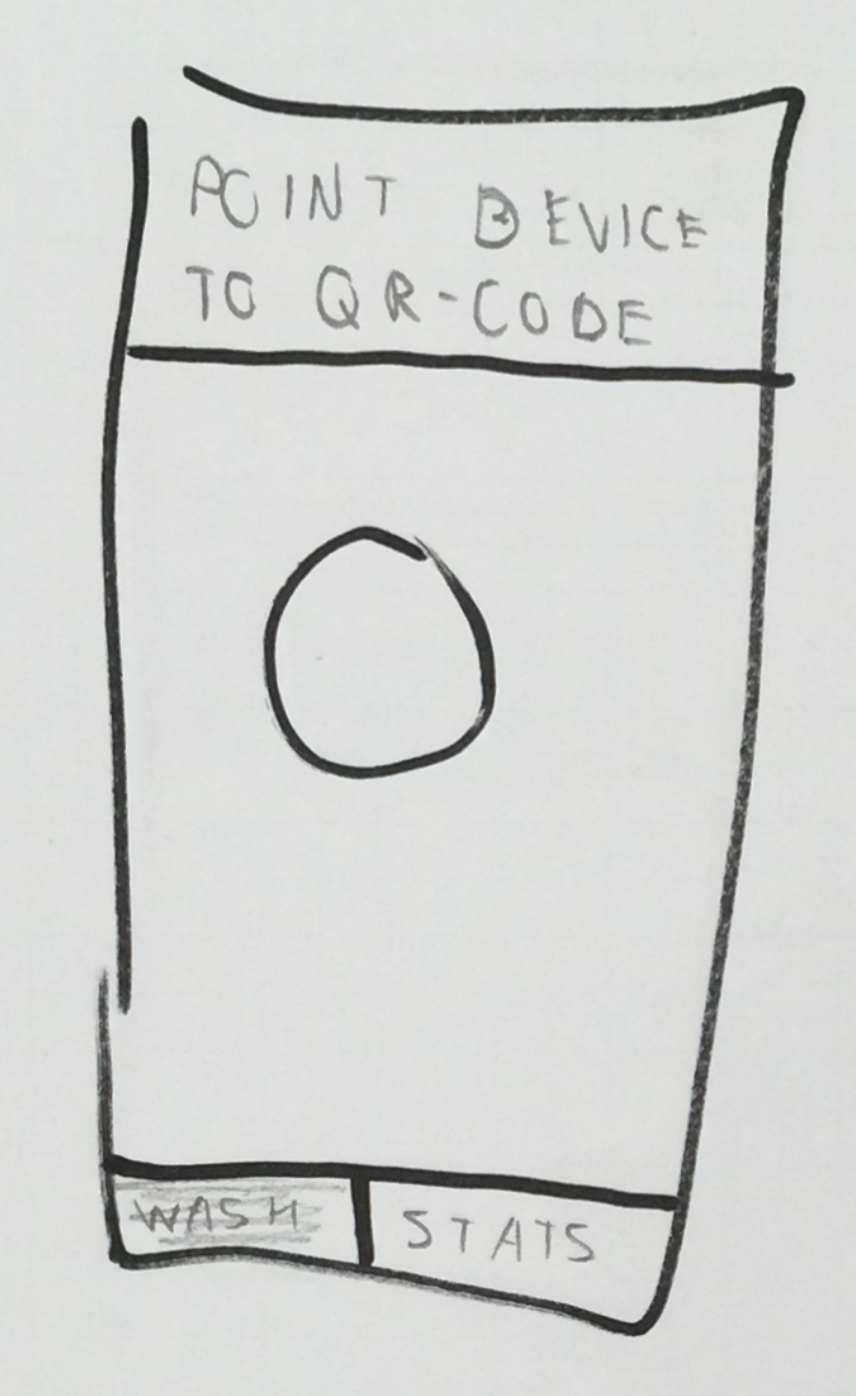
\includegraphics[height=0.5\textwidth]{Bilder/Prot_1.1/Prot_1_1_1.png}
  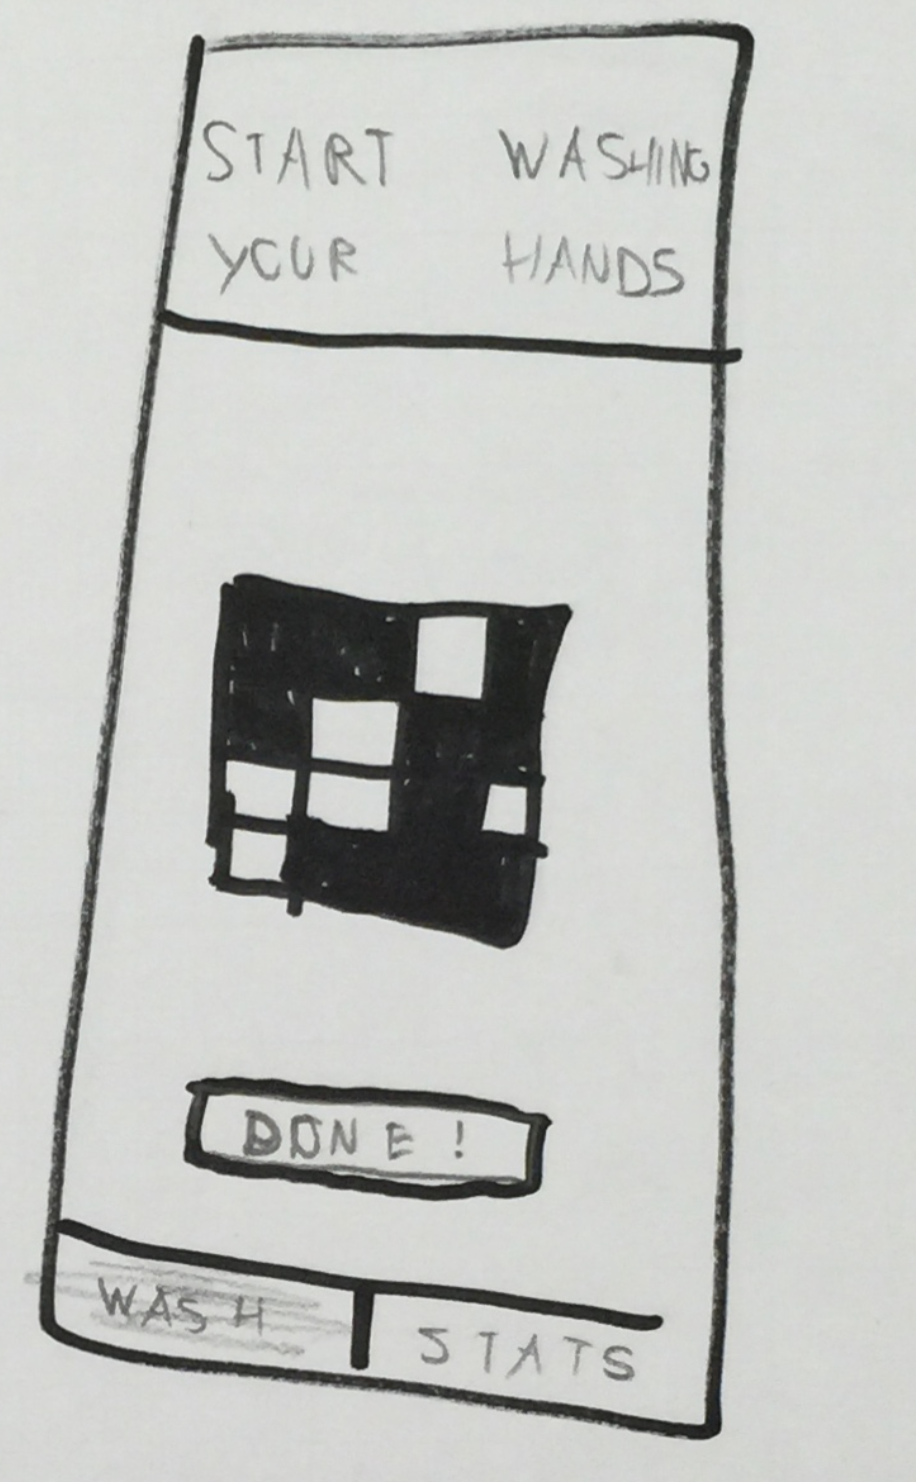
\includegraphics[height=0.5\textwidth]{Bilder/Prot_1.1/Prot_1_1_2.png}
  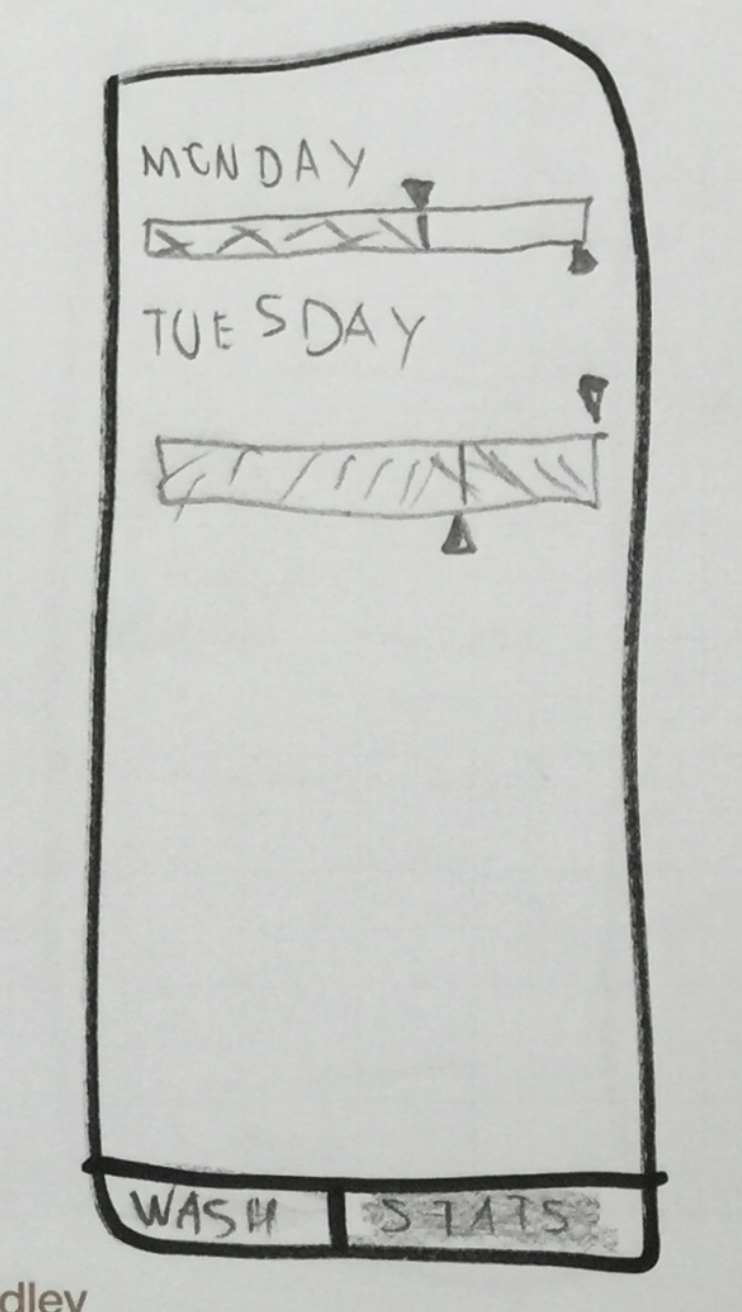
\includegraphics[height=0.5\textwidth]{Bilder/Prot_1.1/Prot_1_1_3.png}
\end{frame}

\begin{frame}
  \frametitle{Prototype 1.2}
  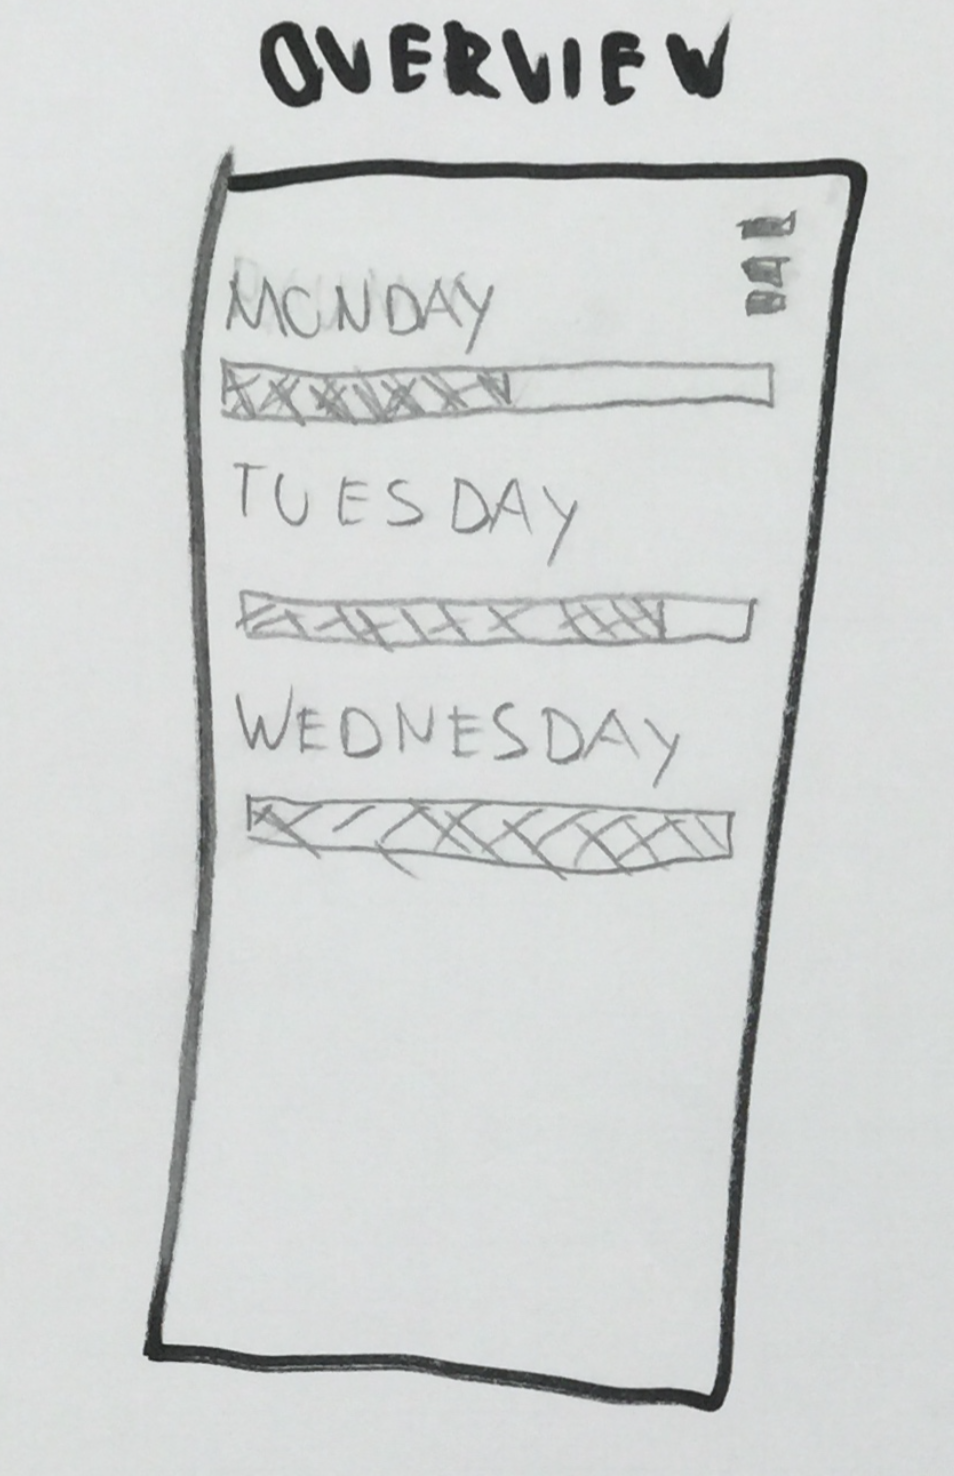
\includegraphics[height=0.5\textwidth]{Bilder/Prot_1.2/Prot_1_2_1.png}
  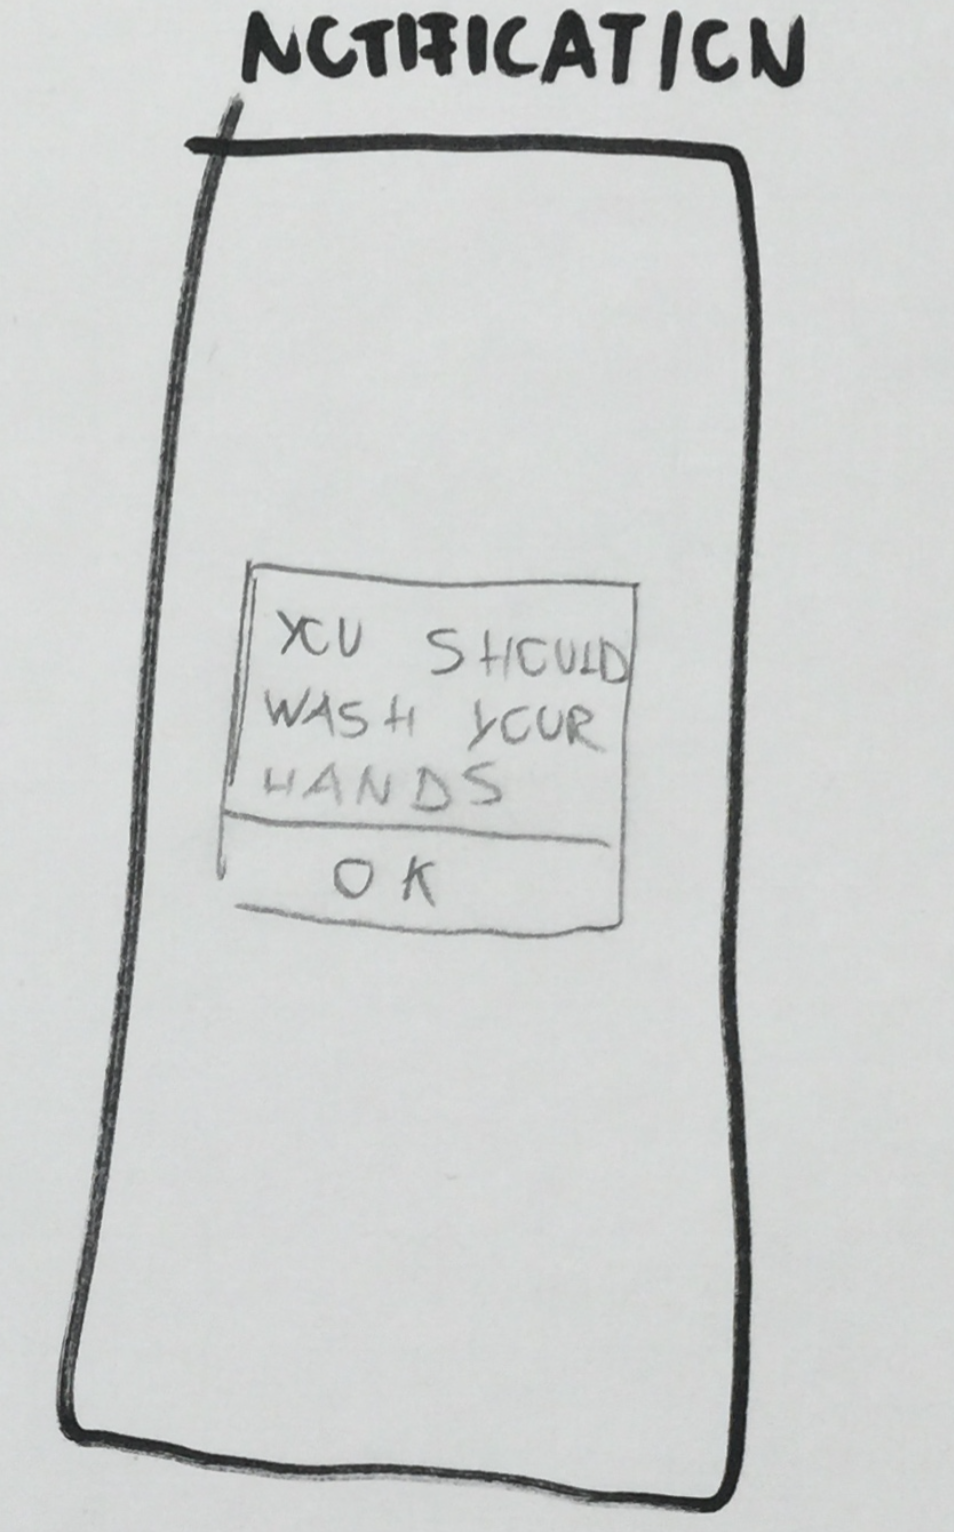
\includegraphics[height=0.5\textwidth]{Bilder/Prot_1.2/Prot_1_2_2.png}
\end{frame}

\begin{frame}
  \frametitle{Prototype 1.2}
  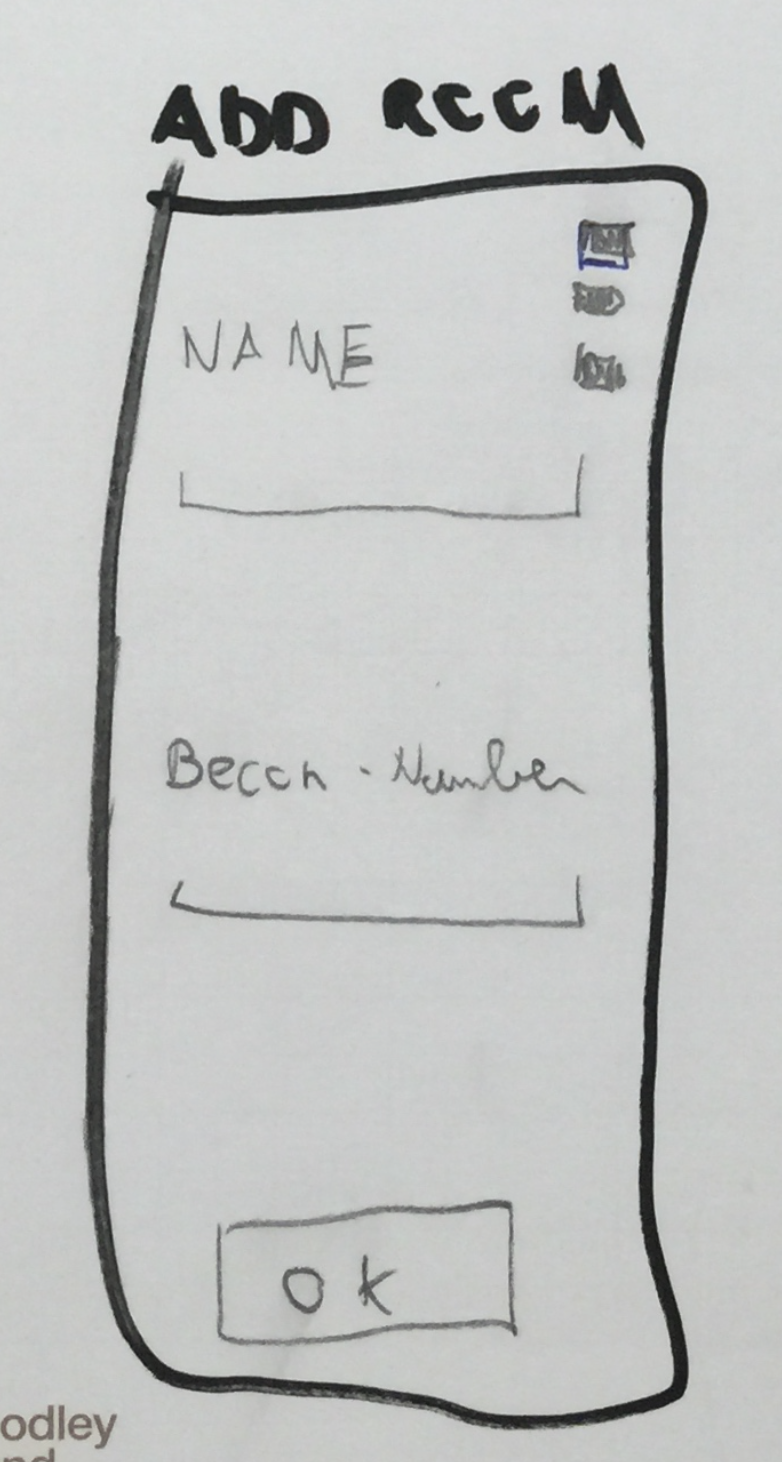
\includegraphics[height=0.5\textwidth]{Bilder/Prot_1.2/Prot_1_2_3.png}
  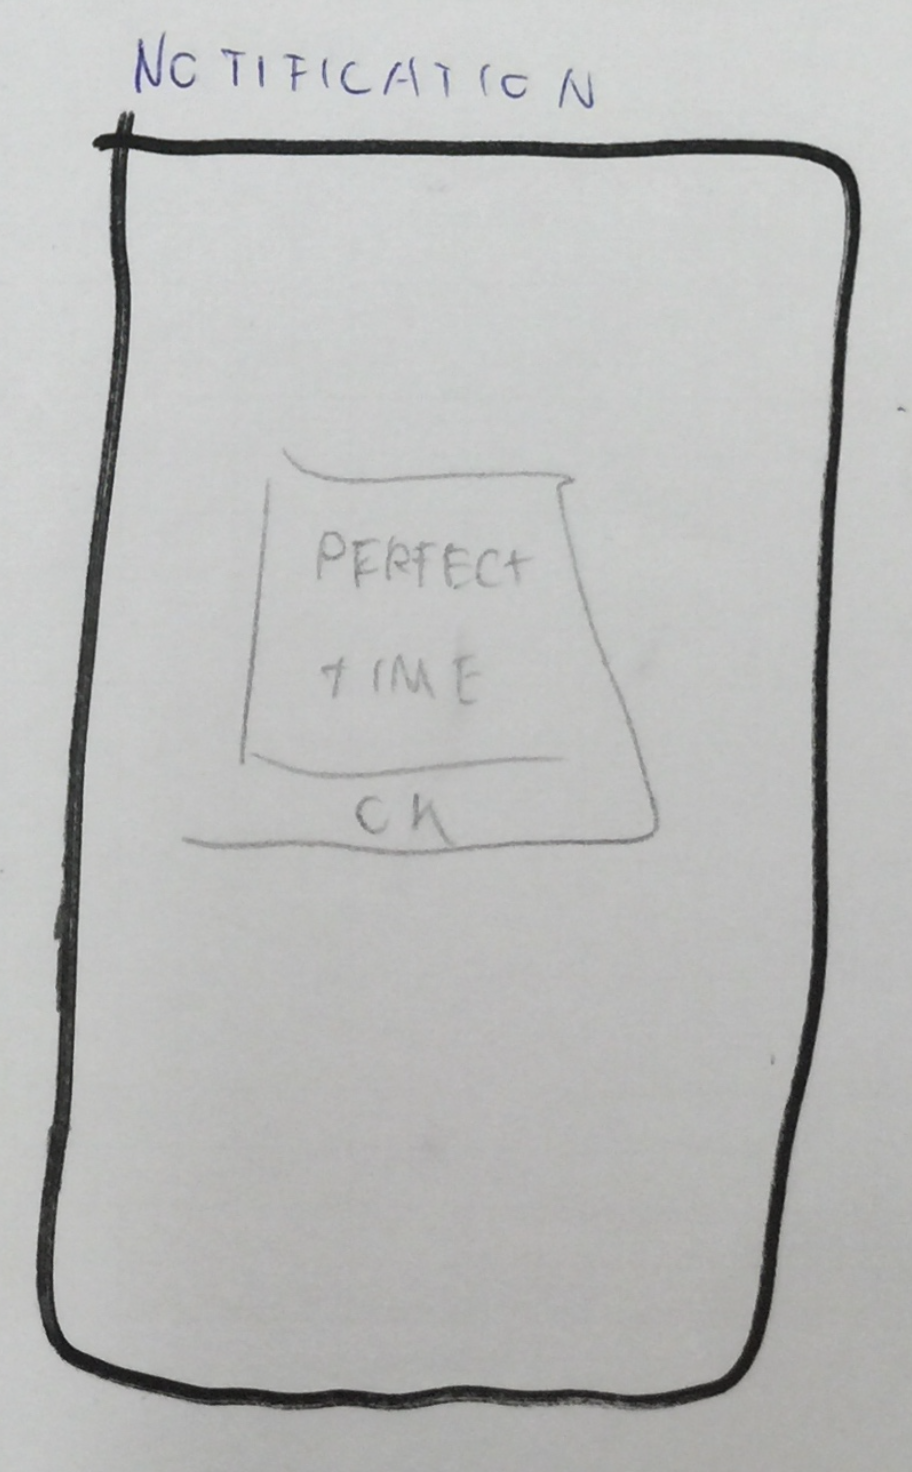
\includegraphics[height=0.5\textwidth]{Bilder/Prot_1.2/Prot_1_2_4.png}
\end{frame}

\begin{frame}
  \frametitle{Prototype 1.3}
  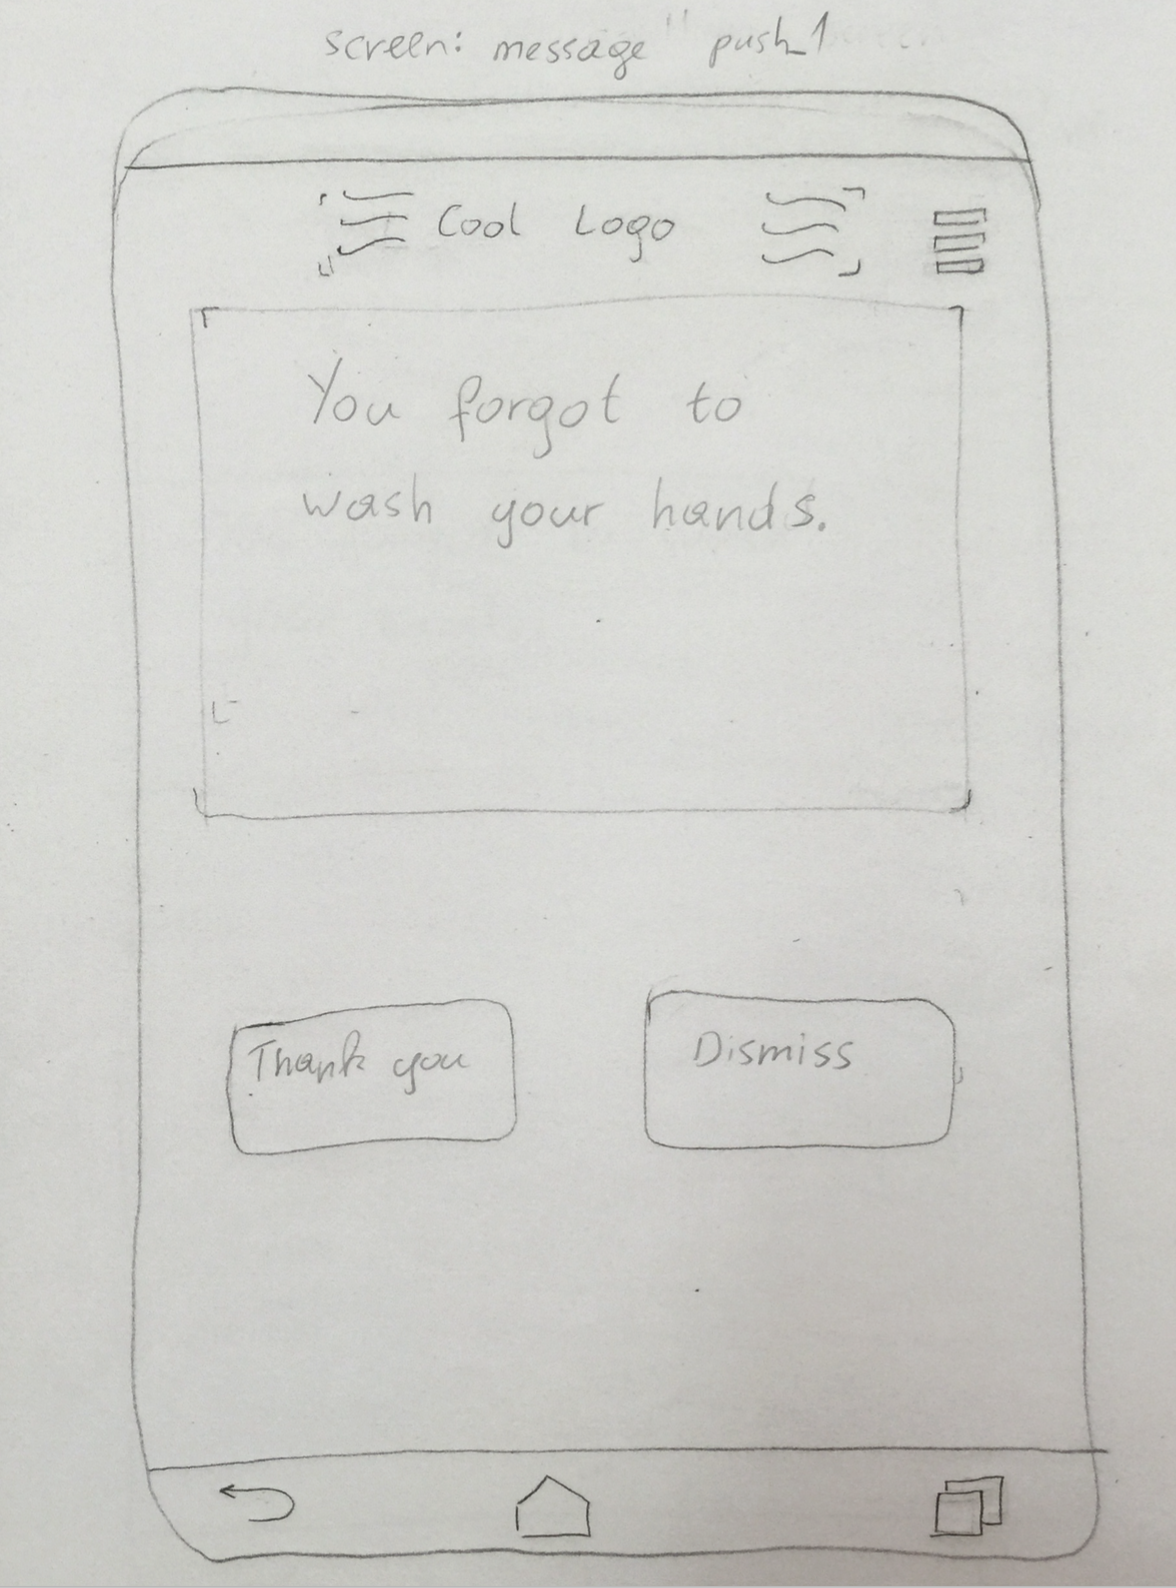
\includegraphics[height=0.5\textwidth]{Bilder/Prot_1.3/Prot_1_3_1.png}
  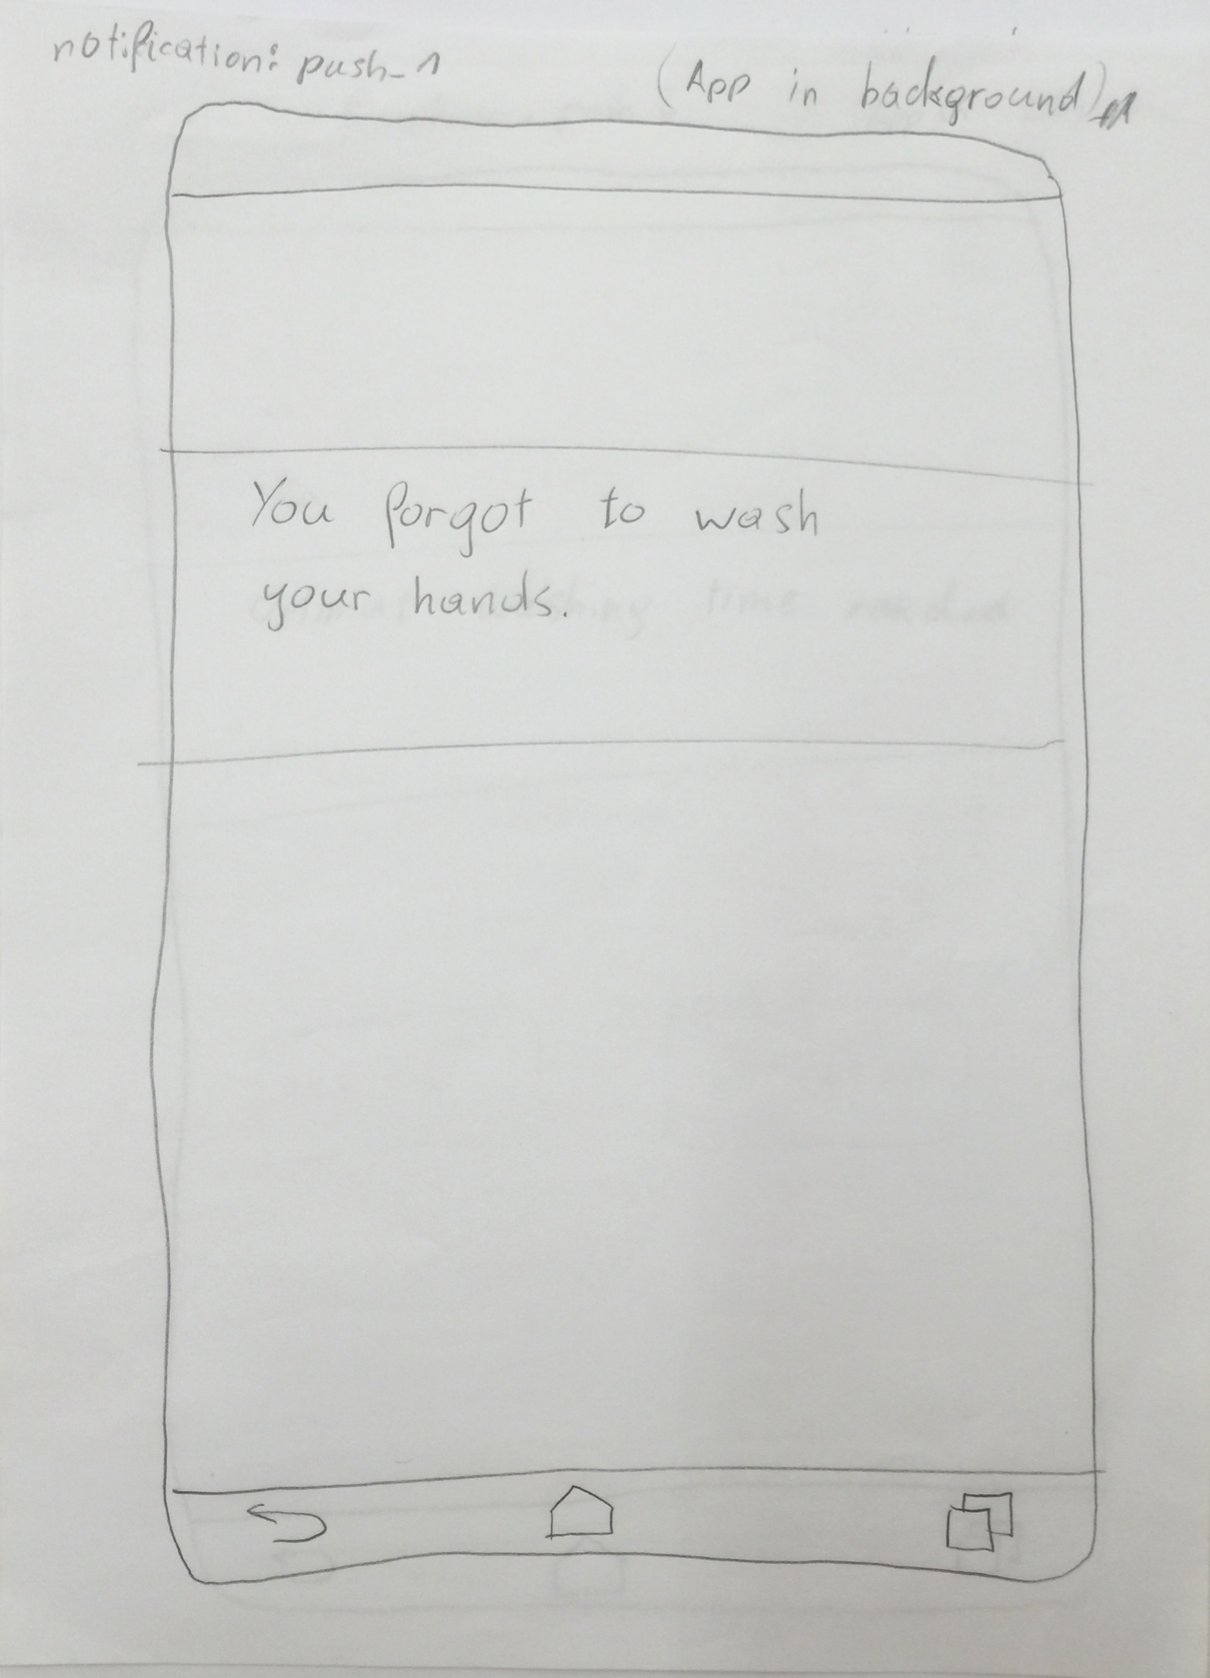
\includegraphics[height=0.5\textwidth]{Bilder/Prot_1.3/Prot_1_3_2.png}
\end{frame}

\begin{frame}
  \frametitle{Prototype 1.3}
  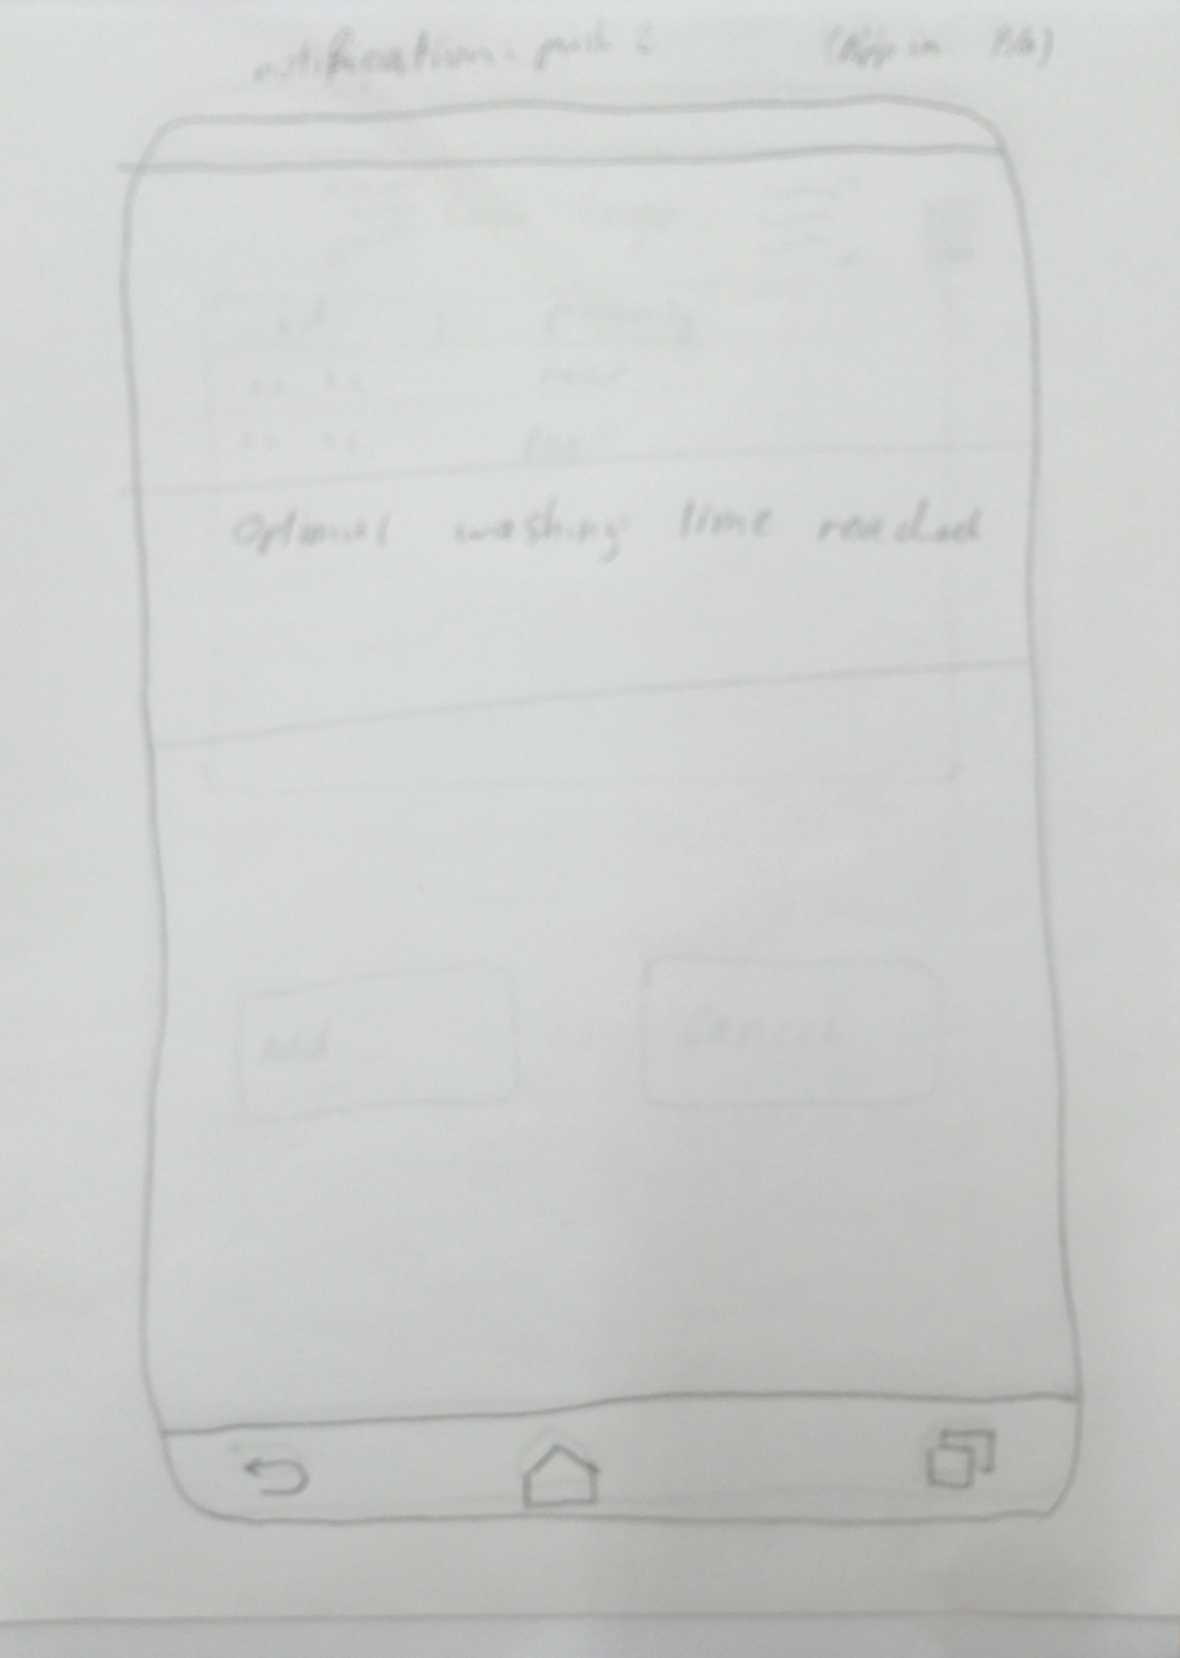
\includegraphics[height=0.5\textwidth]{Bilder/Prot_1.3/Prot_1_3_3.png}
  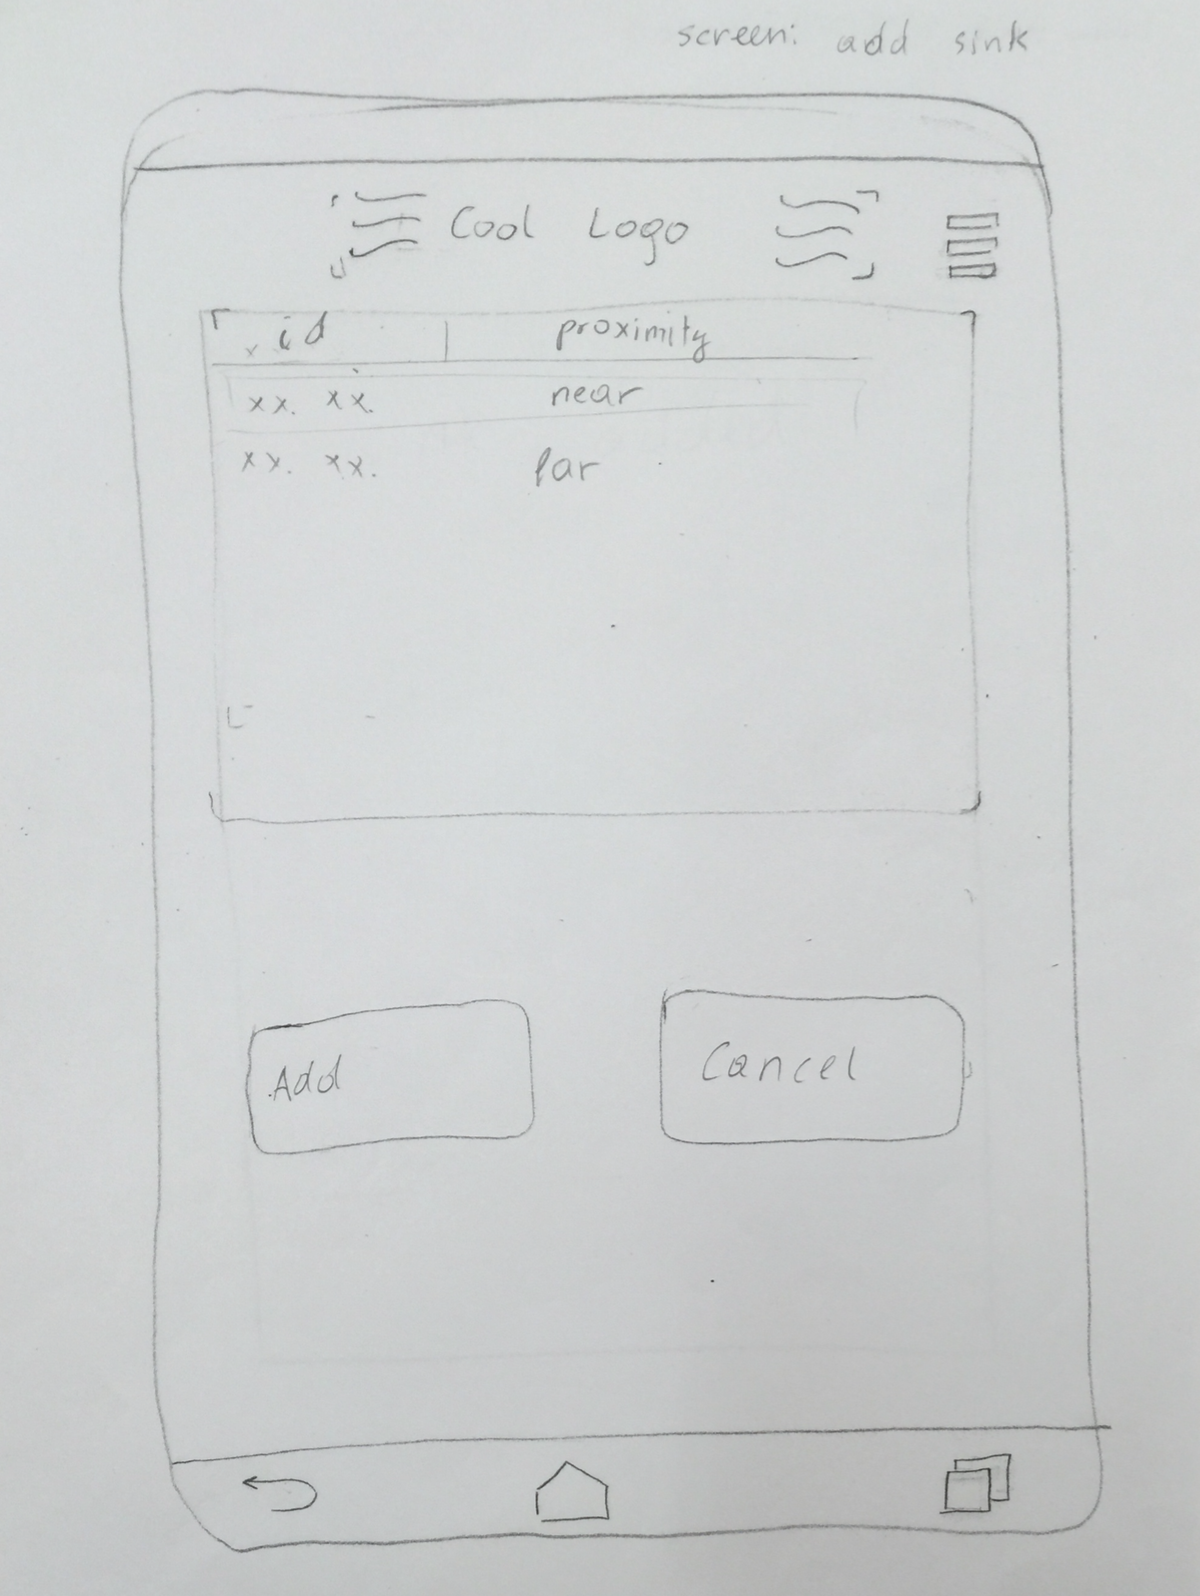
\includegraphics[height=0.5\textwidth]{Bilder/Prot_1.3/Prot_1_3_4.png}
\end{frame}

\begin{frame}
  \frametitle{Prototype 1.3}
  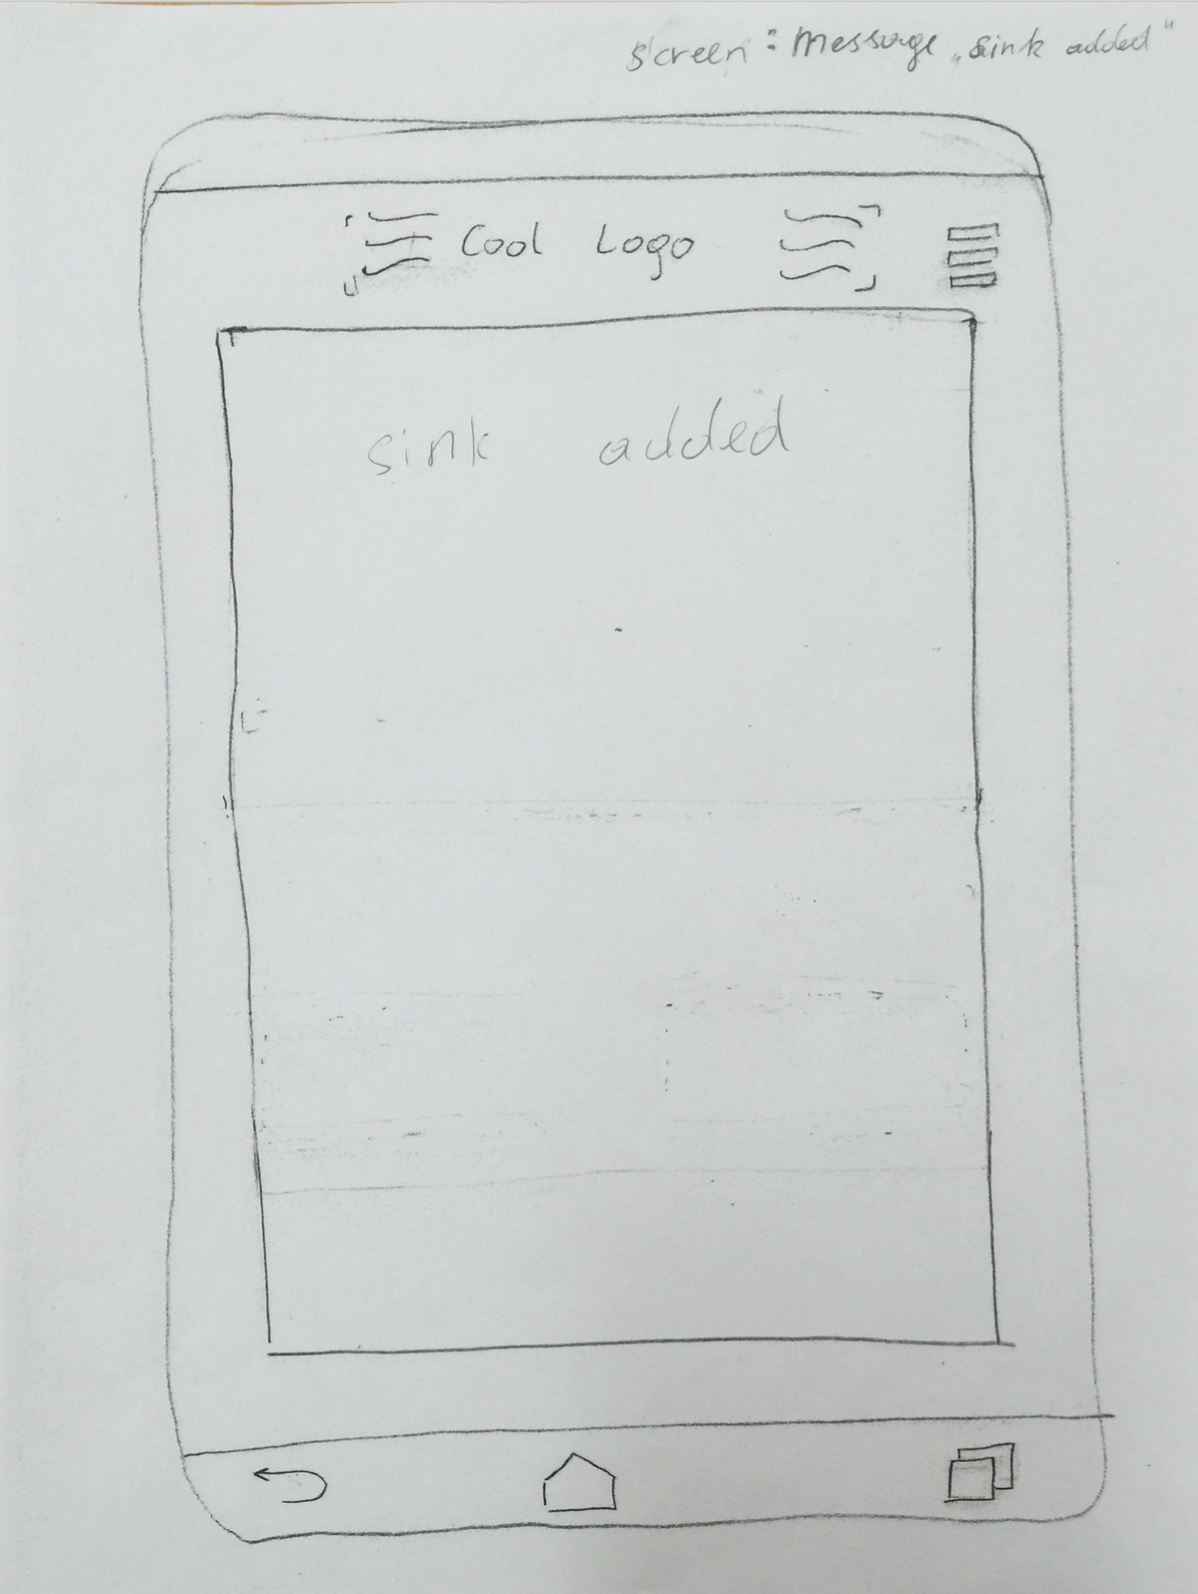
\includegraphics[height=0.5\textwidth]{Bilder/Prot_1.3/Prot_1_3_5.png}
  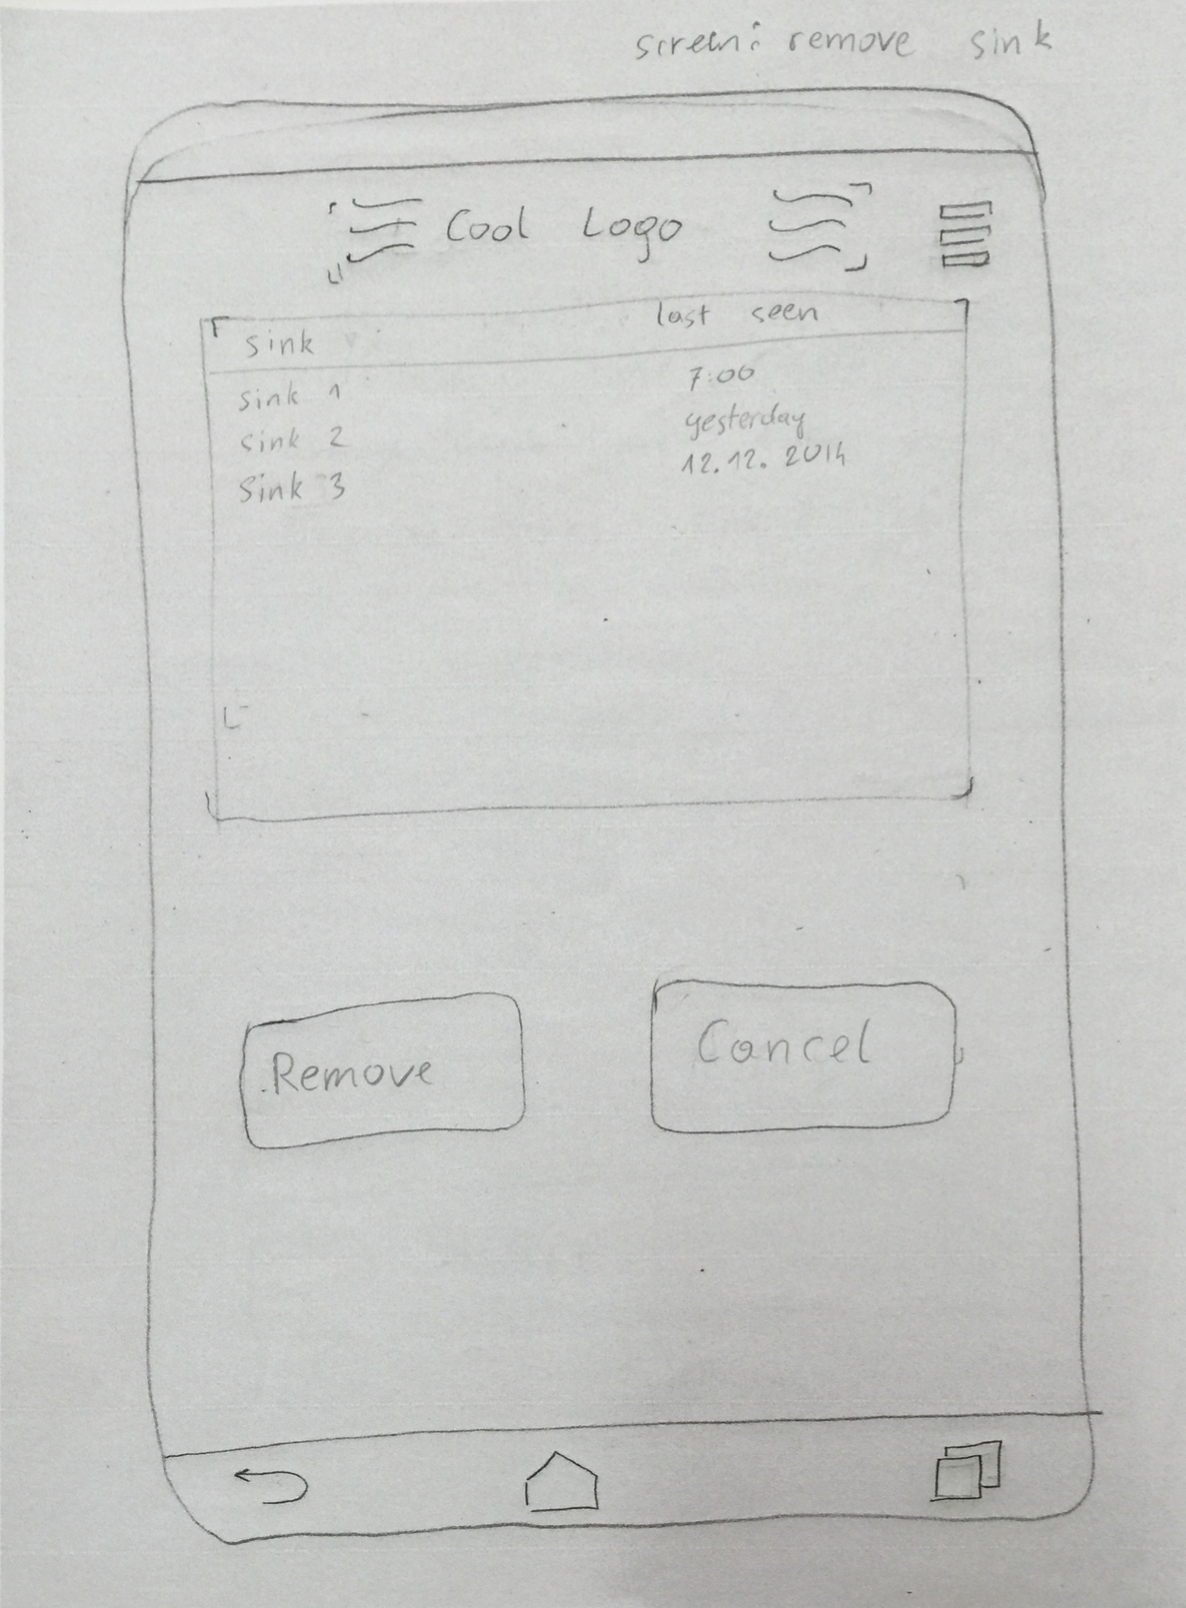
\includegraphics[height=0.5\textwidth]{Bilder/Prot_1.3/Prot_1_3_6.png}
\end{frame}

\begin{frame}
  \frametitle{Prototype 1.3}
  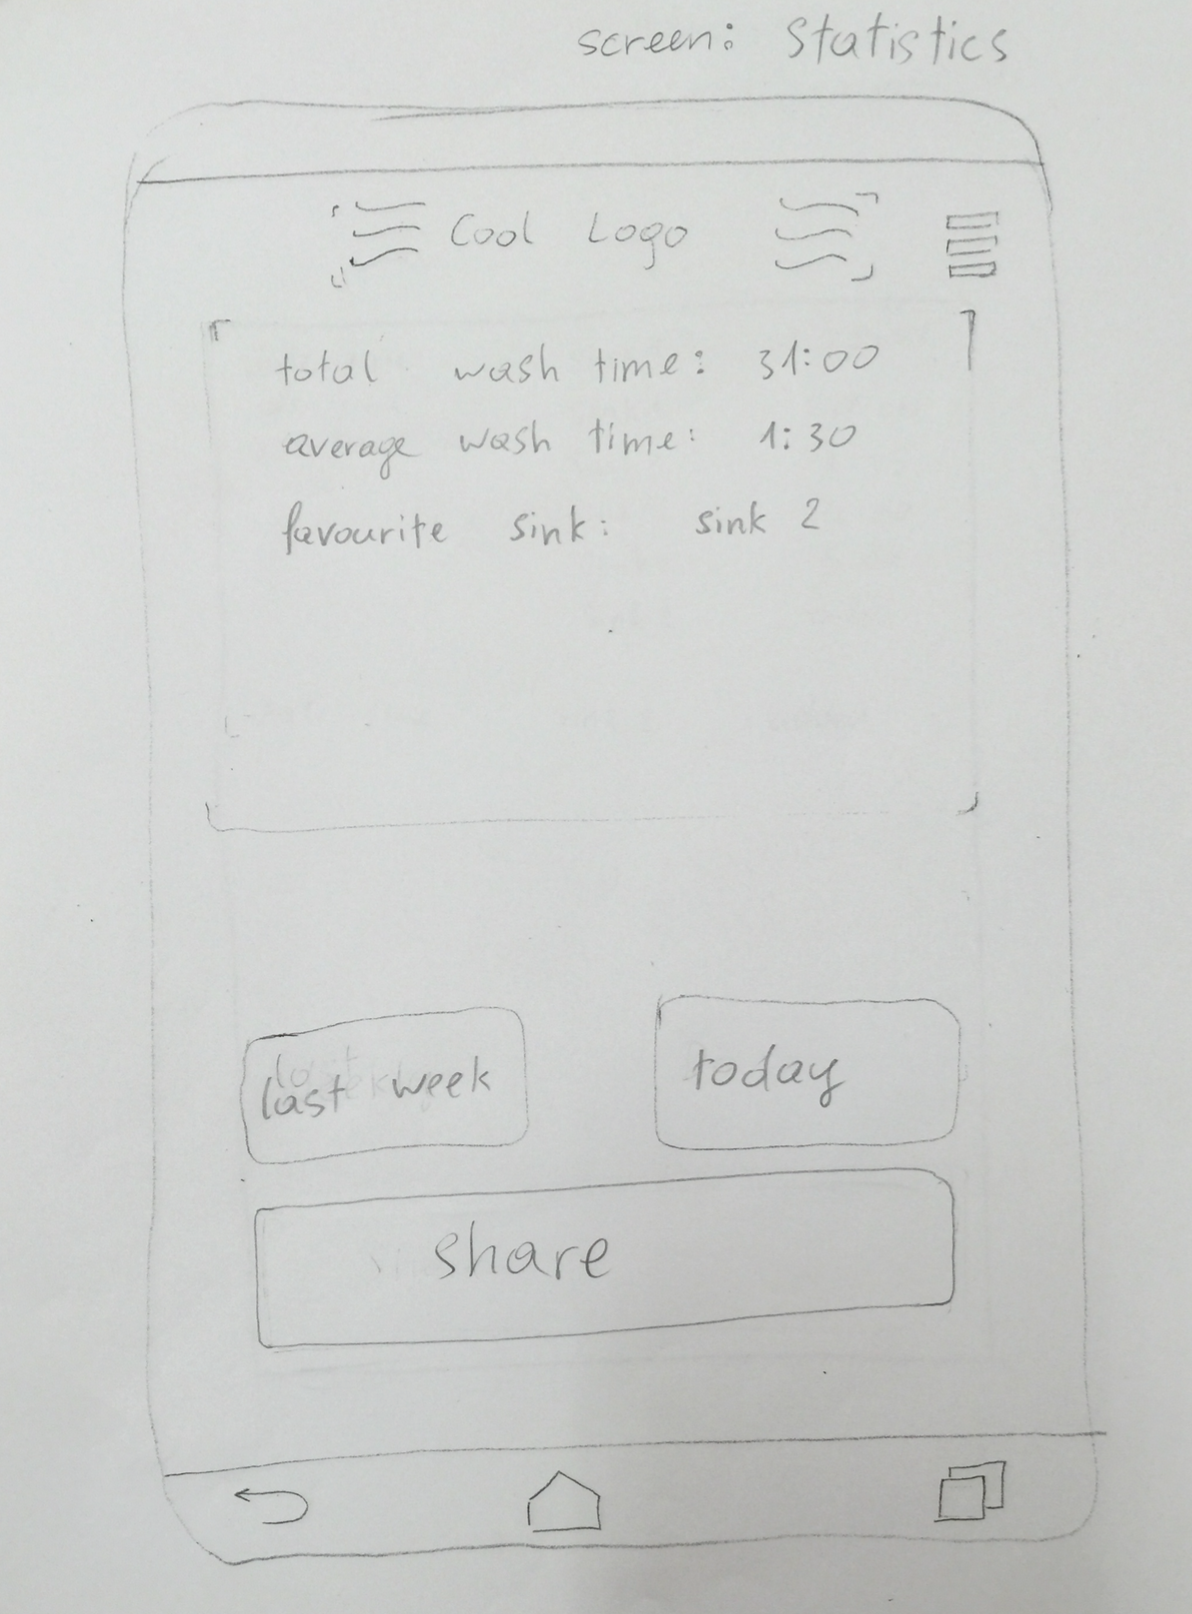
\includegraphics[height=0.5\textwidth]{Bilder/Prot_1.3/Prot_1_3_7.png}
\end{frame}


%%%%%%%%%%%%%%%%%%%%%%%%%%%%%%%%%%%%%%%%%%%%%%%%%%%%%%%%%%%% 
\section{Key Tasks}
%% explain and demonstrate (5 min)
\begin{frame}
  \frametitle{Key Tasks}
  \begin{itemize}
  \item Task 1: Enjoy the optimal handwashing experience
  \item Task 2: Add new room/sink to database
  \end{itemize}          
\end{frame}

\section{User Actions and System Responses}
%% User Actions and System Responses:  Show a complete list
\begin{frame}
  \frametitle{Task 1: wash hands}
  \begin{enumerate}
  \item User: enters bathroom

  \item  \begin{itemize}
    \item User: leaves bathroom
    \item Sys.: Notification: ``You forgot to wash your hands.''
    \end{itemize}

  \item  \begin{itemize}
    \item User: returns to bathroom and washes his hands
    \item Sys.: Notification: ``Optimal handwashing time reached.''
    \end{itemize}
  \end{enumerate}          
\end{frame}

%%------------------------------
\begin{frame}
  \frametitle{Task 2: add sink}
  \begin{enumerate}
  \item	\begin{itemize}
    \item User: Tabs on menu button
    \item Sys.: Shows menu
    \end{itemize}
    
  \item	\begin{itemize}         
    \item User: Tabs at ``add sink''
    \item Sys.: Shows screen: ``Add Sink''
    \end{itemize}
%   \end{enumerate}          
% \end{frame}

% \begin{frame}
%   \frametitle{Task 2: add sink}
%   \begin{enumerate} \setcounter{enumi}{2}
    
  \item	\begin{itemize}
    \item User: Selects beacon
    \item Sys.: Higlights selected item
    \end{itemize}
    
  \item	\begin{itemize}         
    \item User: Presses ``Add'' button
    \item Sys.: Shows message ``Sink added''
    \end{itemize}          
  \end{enumerate}
\end{frame}


%%%%%%%%%%%%%%%%%%%%%%%%%%%%%%%%%%%%%%%%%%%%%%%%%%%%%%%%%%%%
\section{Cognitive Walkthrough}
%% assessment of CW questions: show complete list, explain two examples (1 min)
\begin{frame}
  \frametitle{Cognitive Walkthrough - Questions}
  \begin{enumerate}
  \item Does the effect of the user's interaction with the system match the goal of the action?
  \item Does the user see that an action is available?
  \item Can the user recognize that the action is the right one?
  \item After action, can the user understand the system's feedback?
  \end{enumerate}
\end{frame}

%% ------------------------------
\begin{frame}
  \frametitle{Cognitive Walkthrough - Task 1}
  1. User enters bathroom

  \begin{tabular}{ll}
    Effect matches goal?     & Yes \\
    Action visible?          & Yes \\
    Action recognizable?     & Yes \\
    Feedback understandable? & No feedback by design \\
  \end{tabular}
\end{frame}


\begin{frame}
  \frametitle{Cognitive Walkthrough - Task 1}
  2. User leaves bathroom without washing his hands 




  \begin{tabular}{ll}
    Effect matches goal?     & Yes \\
    Action visible?          & Yes \\
    Action recognizable?     & Yes \\
    Feedback understandable? & Yes \\
  \end{tabular}
\end{frame}

\begin{frame}
  \frametitle{Cognitive Walkthrough - Task 1}
  3. User washes hands 


  \begin{tabular}{ll}
    Effect matches goal?     & Yes \\
    Action visible?          & Yes \\
    Action recognizable?     & Yes \\
    Feedback understandable? & Yes \\
  \end{tabular}
\end{frame}

%%------------------------------
\begin{frame}
  \frametitle{Cognitive Walkthrough - Task 2}
  1. open menu 


  \begin{tabular}{ll}
    Effect matches goal?     & Yes \\
    Action visible?          & Yes \\
    Action recognizable?     & Yes \\
    Feedback understandable? & Yes \\
  \end{tabular}
\end{frame}

\begin{frame}
  \frametitle{Cognitive Walkthrough - Task 2}
  2. select ``add sink'' 


  \begin{tabular}{ll}
    Effect matches goal?     & Yes \\
    Action visible?          & Yes \\
    Action recognizable?     & Yes \\
    Feedback understandable? & No (no headline) \\
  \end{tabular}
\end{frame}

\begin{frame}
  \frametitle{Cognitive Walkthrough - Task 2}
  3. select beacon


  \begin{tabular}{ll}
    Effect matches goal?     & Yes \\
    Action visible?          & No (list selectable?) \\
    Action recognizable?     & No (which one?) \\
    Feedback understandable? & Yes \\
  \end{tabular}
\end{frame}

\begin{frame}
  \frametitle{Cognitive Walkthrough - Task 2}
  4. Presses ``Add'' button 


  \begin{tabular}{ll}
    Effect matches goal?     & Yes \\
    Action visible?          & Yes \\
    Action recognizable?     & Yes \\
    Feedback understandable? & Yes \\
  \end{tabular}
\end{frame}




%%%%%%%%%%%%%%%%%%%%%%%%%%%%%%%%%%%%%%%%%%%%%%%%%%%%%%%%%%%%
\section{Changes}
%% Explain the key changes that you made to the design (4 min)
\begin{frame}
  \frametitle{Key Changes}
  \begin{itemize}
  \item automatic choose the closest beacon to add
  \item allow user name beacons
  \item integrate headline in titlebar
  \end{itemize}          
\end{frame}


%%%%%%%%%%%%%%%%%%%%%%%%%%%%%%%%%%%%%%%%%%%%%%%%%%%%%%%%%%%%
\section{Final Prototype}
%% DEMO (5 min)
\begin{frame}
  \frametitle{Final Prototype}
  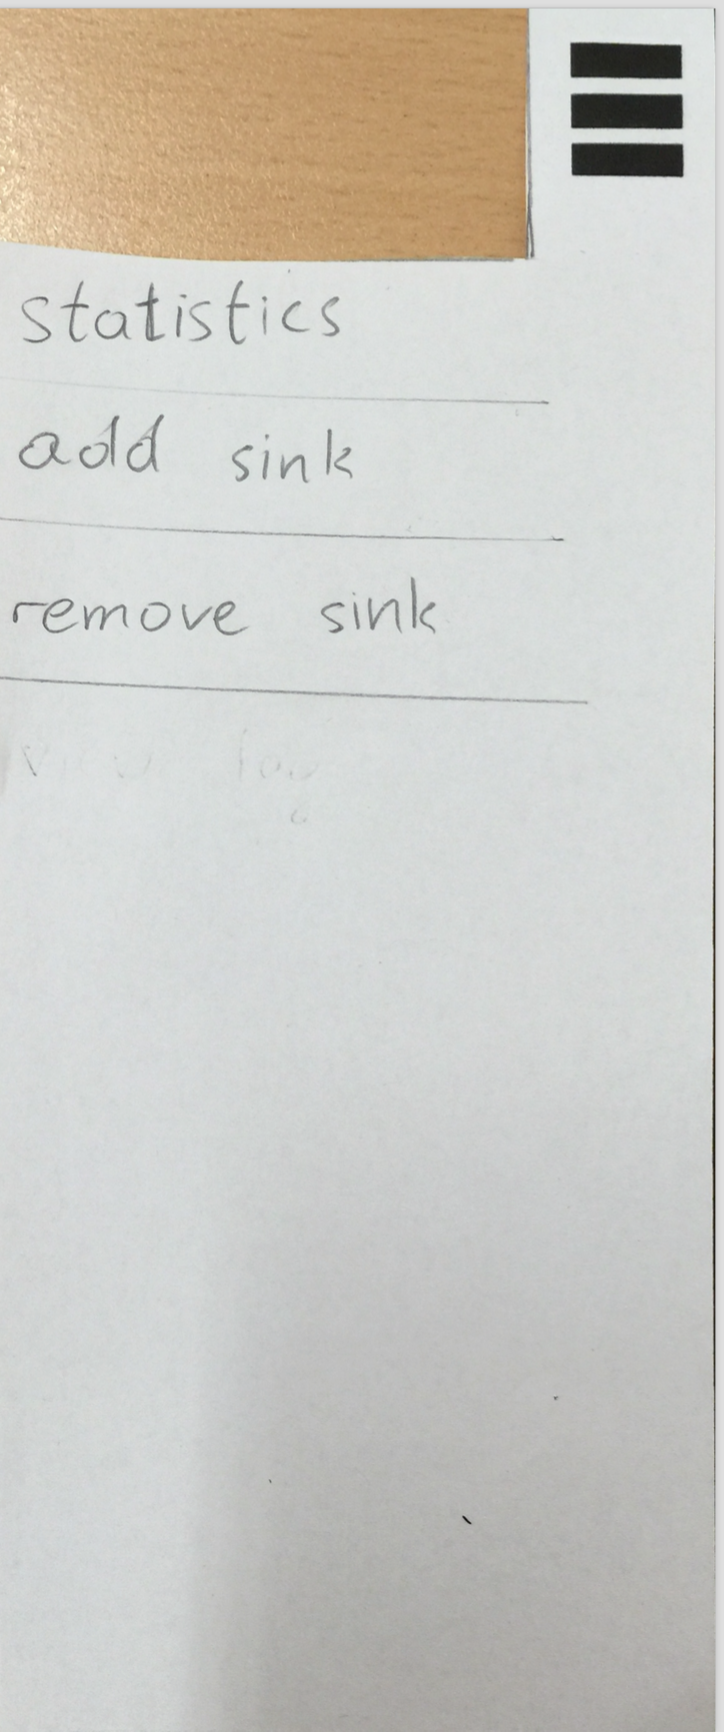
\includegraphics[height=0.4\textwidth]{Bilder/Prot_2.1/Prot_2_1_1.png}
  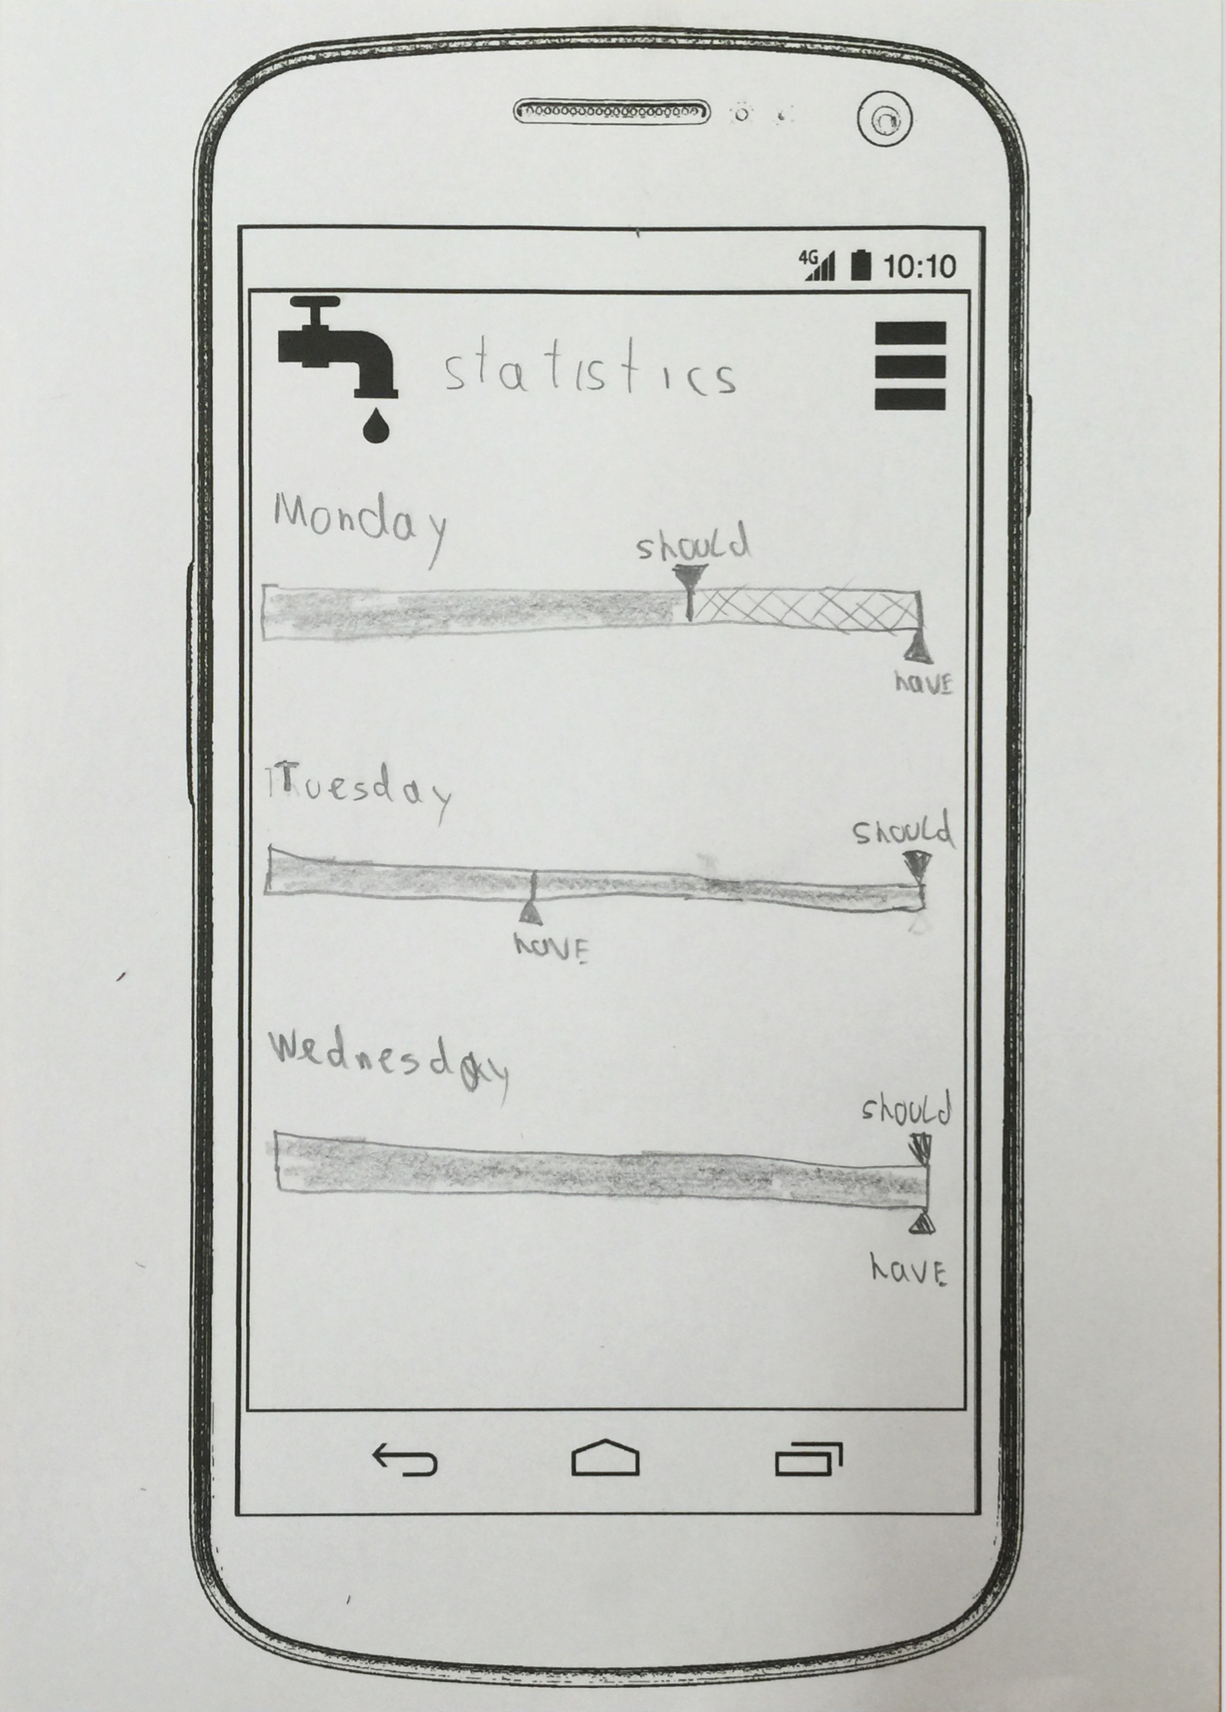
\includegraphics[height=0.5\textwidth]{Bilder/Prot_2.1/Prot_2_1_2.png}
  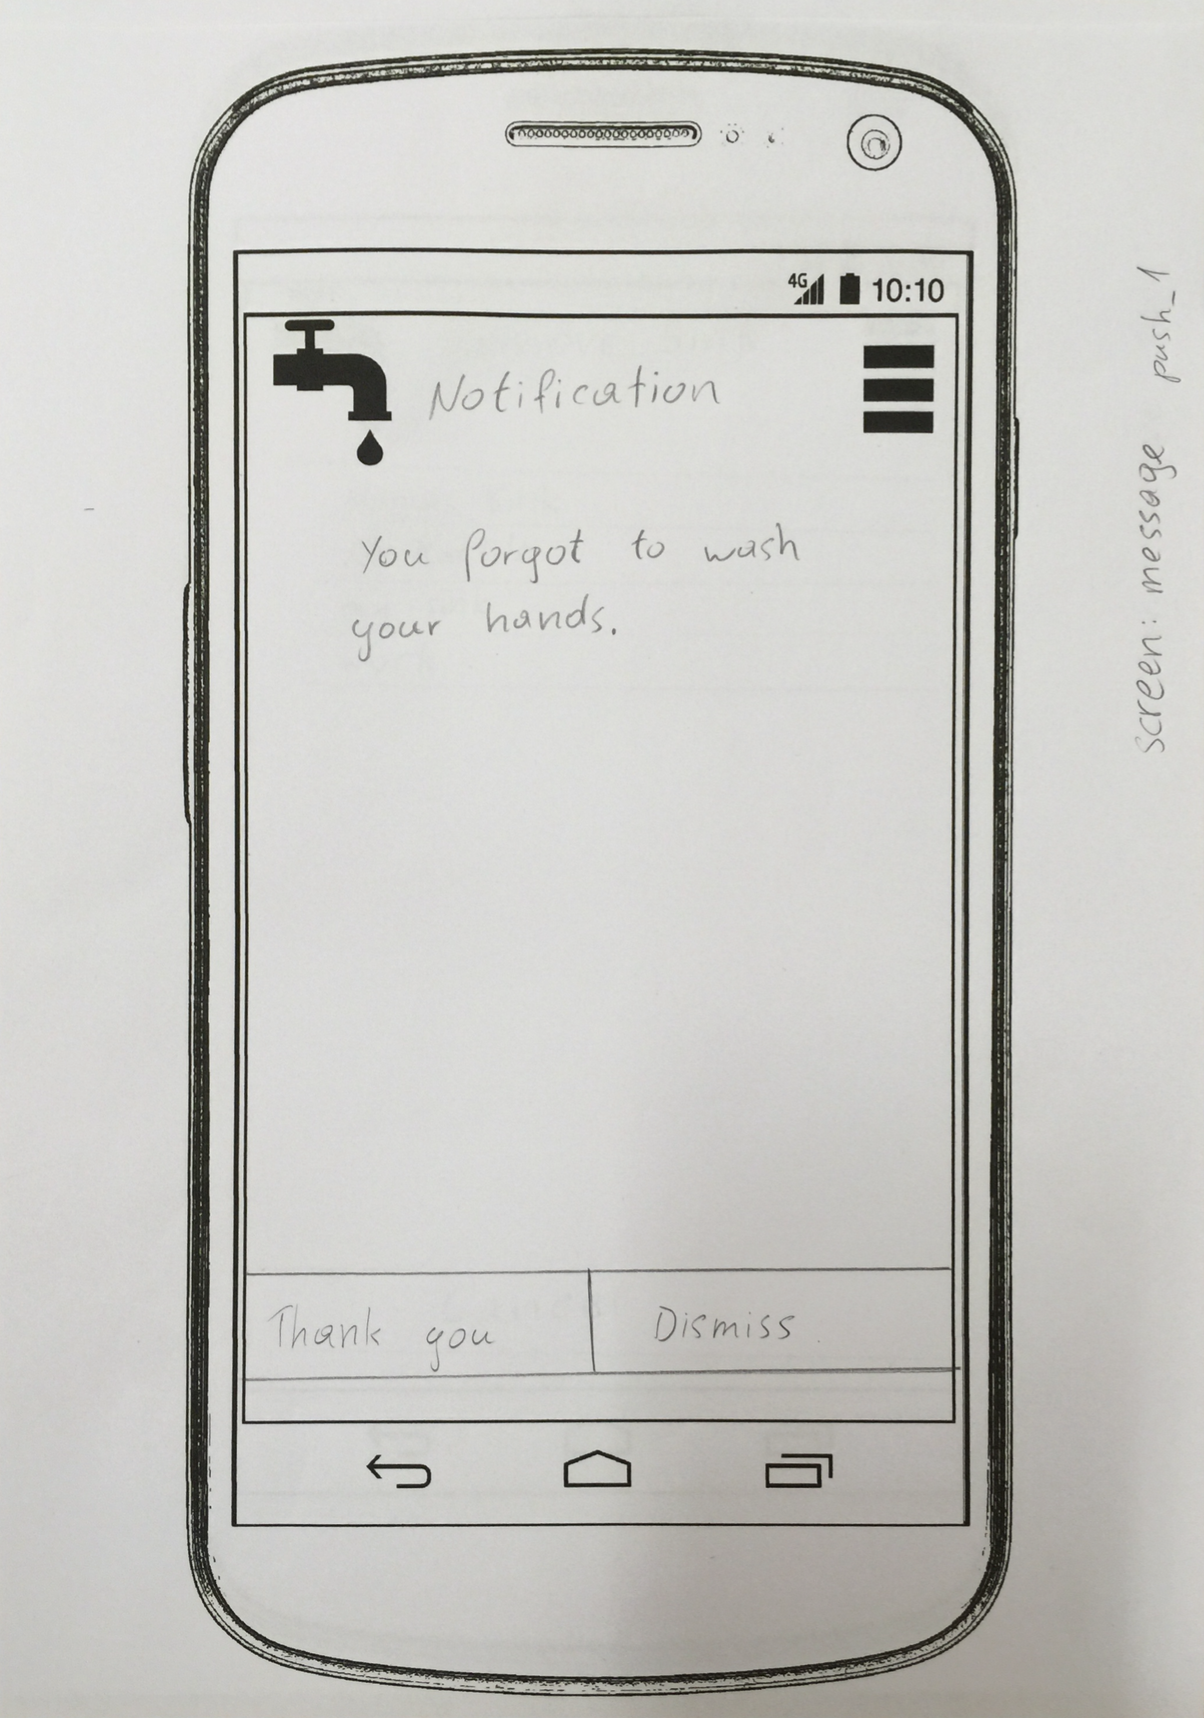
\includegraphics[height=0.5\textwidth]{Bilder/Prot_2.1/Prot_2_1_3.png}
\end{frame}

\begin{frame}
  \frametitle{Final Prototype}
  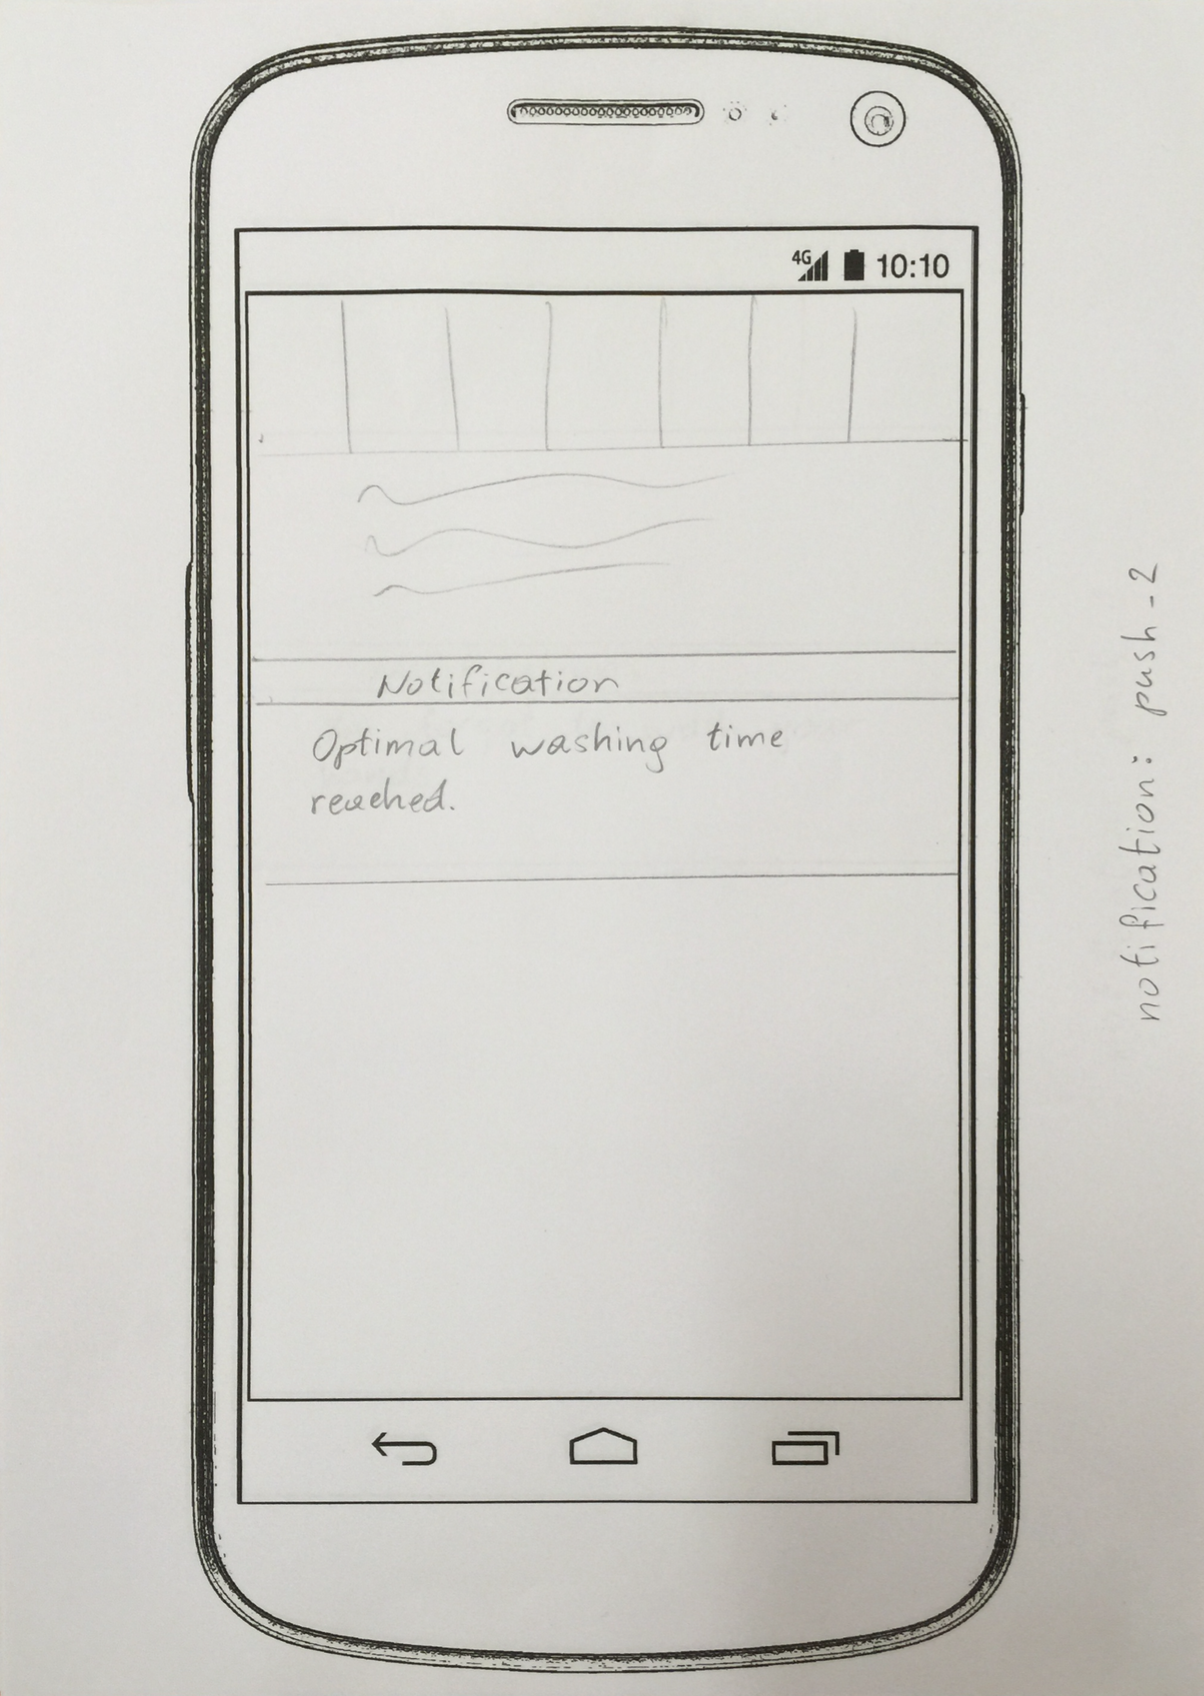
\includegraphics[height=0.5\textwidth]{Bilder/Prot_2.1/Prot_2_1_4.png}
  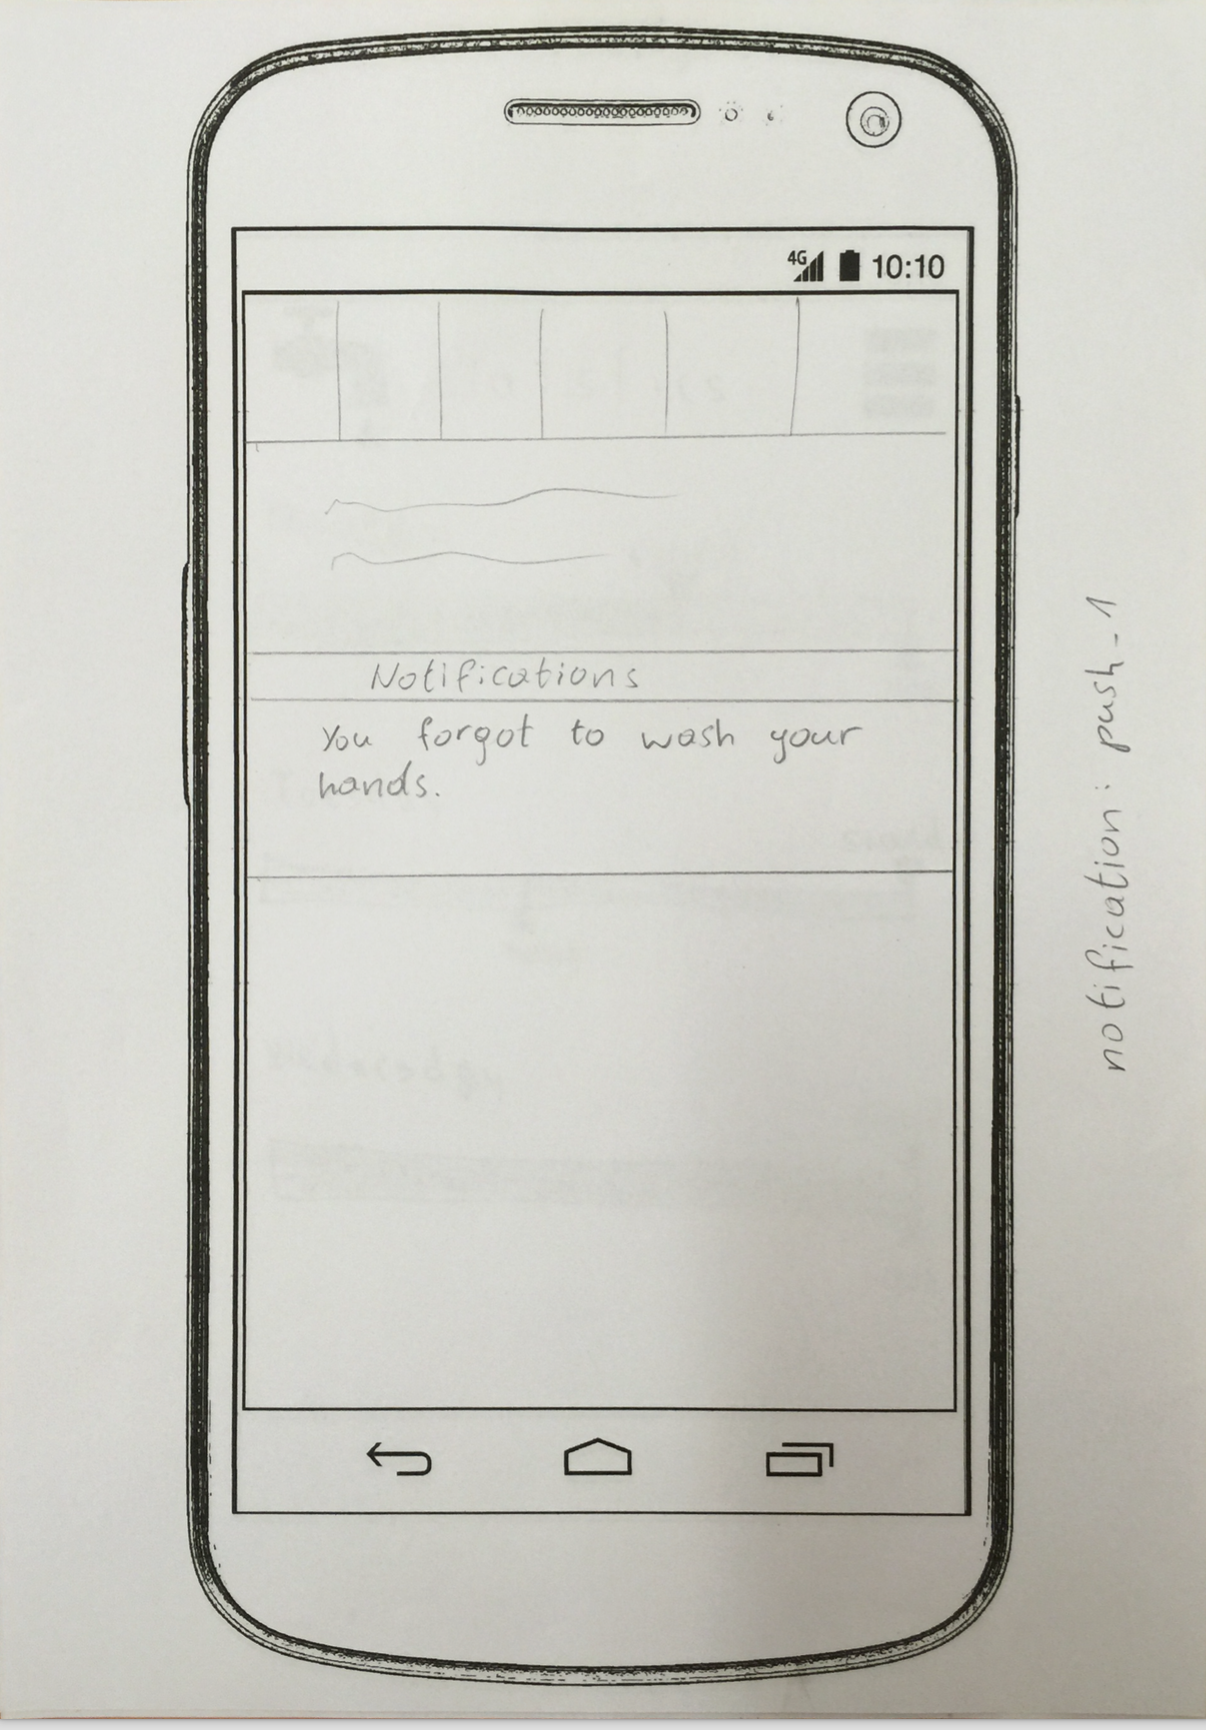
\includegraphics[height=0.5\textwidth]{Bilder/Prot_2.1/Prot_2_1_5.png}
\end{frame}

\begin{frame}
  \frametitle{Final Prototype}
  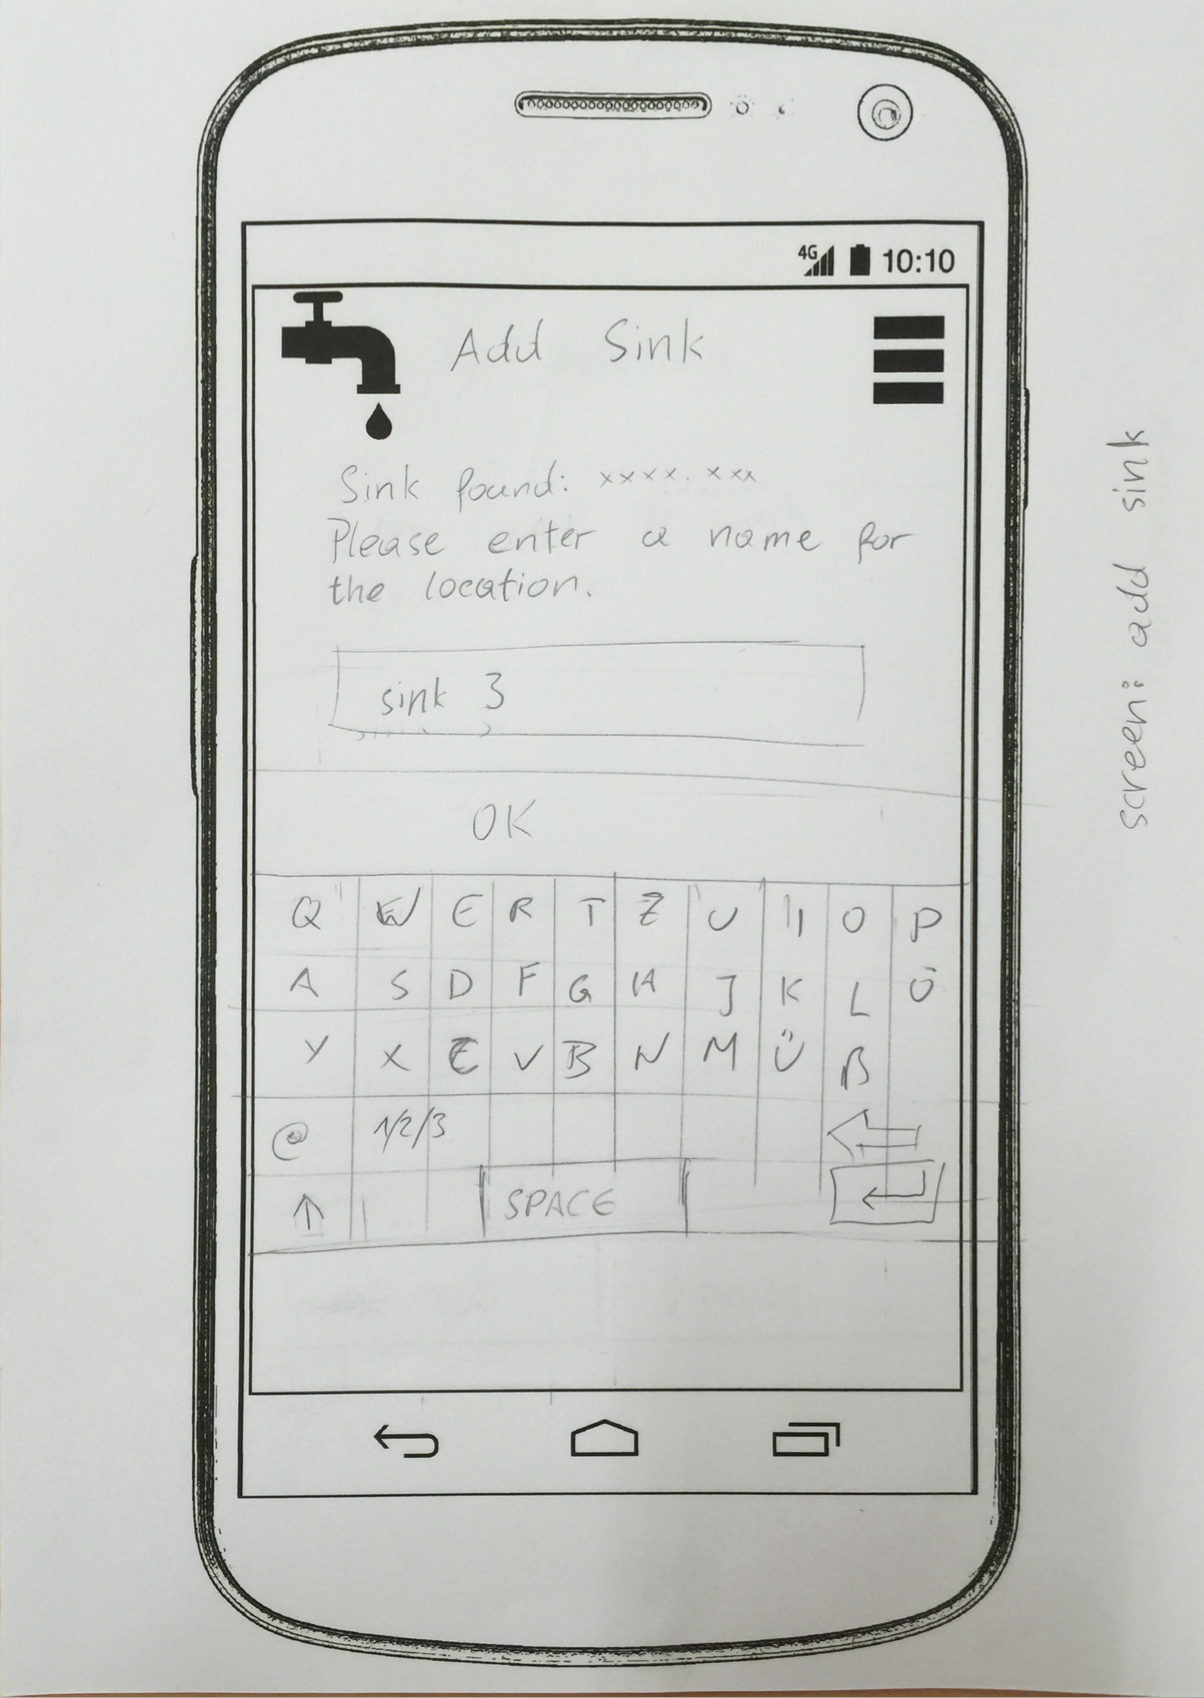
\includegraphics[height=0.5\textwidth]{Bilder/Prot_2.1/Prot_2_1_6.png}
  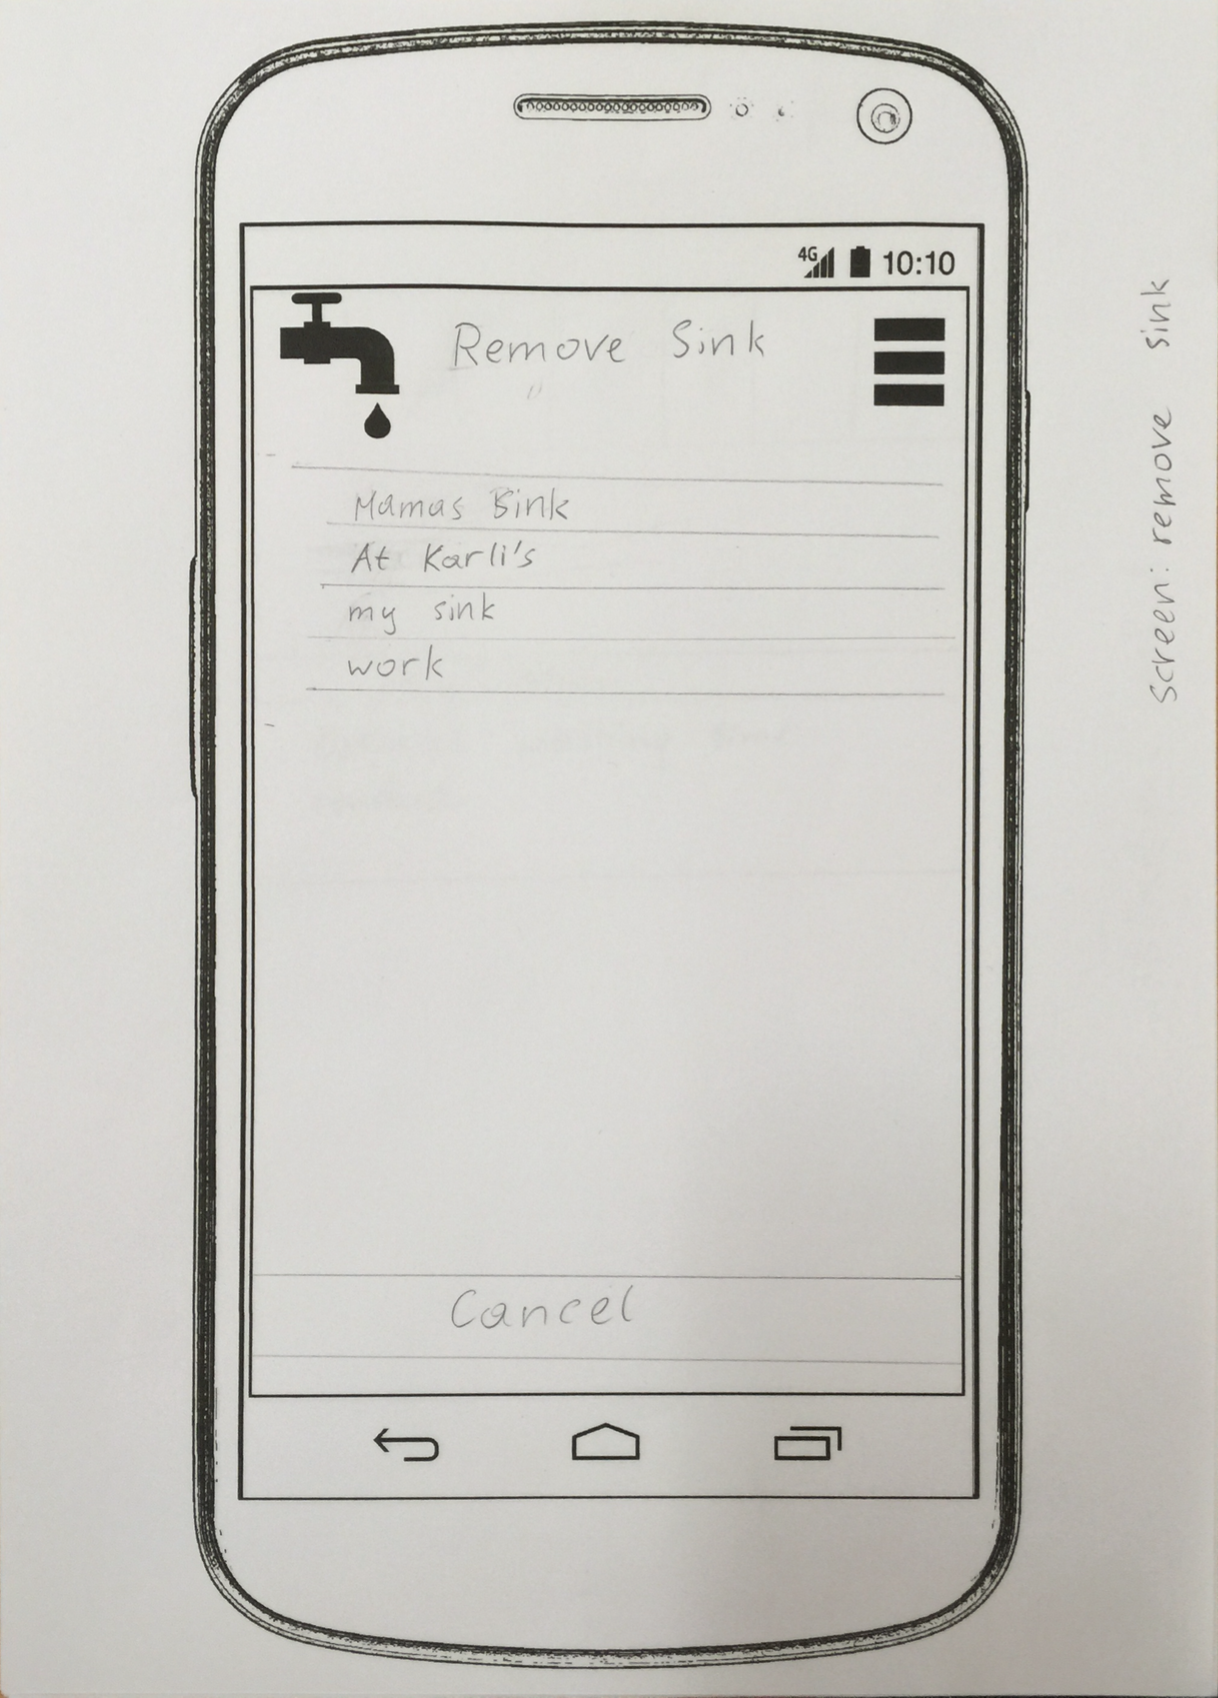
\includegraphics[height=0.5\textwidth]{Bilder/Prot_2.1/Prot_2_1_7.png}
\end{frame}



%%%%%%%%%%%%%%%%%%%%%%%%%%%%%%%%%%%%%%%%%%%%%%%%%%%%%%%%%%%%%%%%%%%%%%%%%%%%
\end{document}
%%%%%%%%%%%%%%%%%%%%%%%%%%%%%%%%%%%%%%%%%%%%%%%%%%%%%%%%%%%%%%%%%%%%%%%%%%%%

%% EOF
